% CHAPITRE 2
% SUIVI VARIABILITE SPATIALE

\chapter{Sites d'études et méthodologies employées}

\minitoc

\newpage

\section{Présentation du site d'étude}

\begin{figure}
\centering
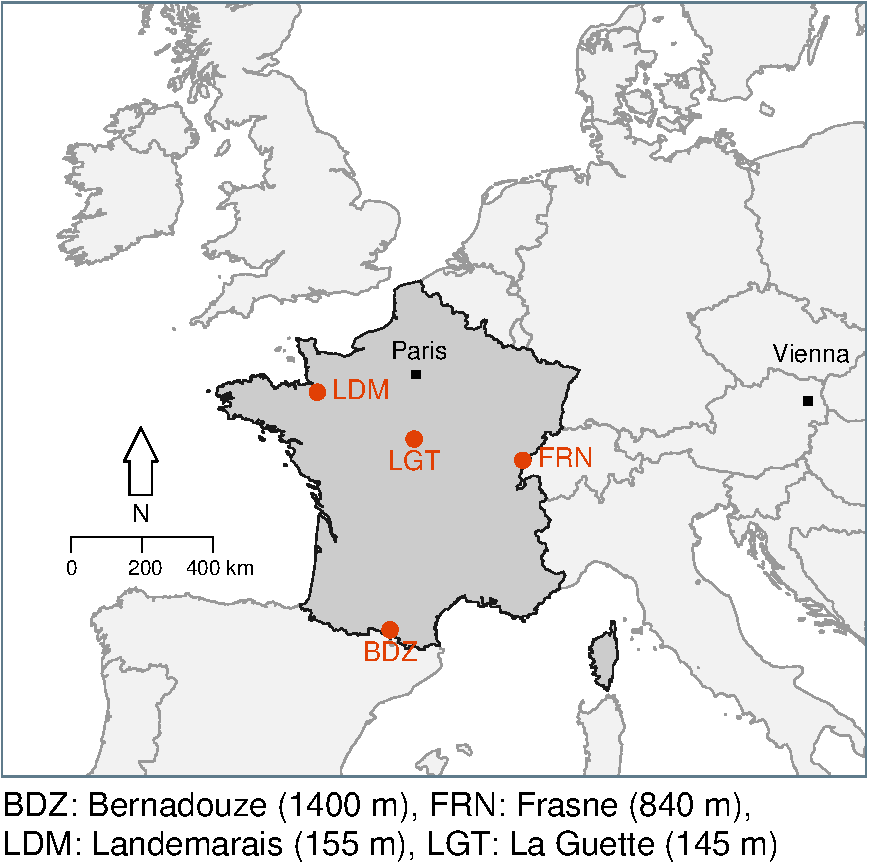
\includegraphics[width=.75\textwidth]{chap2/SNO_siteLocalisation}
\caption{Site d'études SNO}
\label{fig:carte_europe}
\end{figure}

\begin{figure}
\includegraphics[width=\textwidth]{chap2/carteGLc}
\caption{Carte de la tourbière de La Guette}
\label{fig:carte_LG}
\end{figure}


L'ensemble des sites d'études sont regroupés au sein d'un service d'observation

%\subsection{La Guette}

La tourbière de La Guette est situé à Neuvy-sur-Barangeon, en Sologne, dans le département du Cher.
Le site s'étend sur une surface d'une vingtaine d'hectare avec une géométrie relativement allongée.
Avec une conductivité généralement inférieur à 80 uS/m2 et un pH compris entre 4 et 5 elle se classe parmis les "transitionnal poor fen"
Les datations effectuées sur le site permettent de dire que la tourbière est agée de 5 à 6000 ans.
Dans les années 19XX la construction d'une route coupe la tourbière dans sa partie sud.
En 2008 le récurage du fossé de drainage bordant la route semble entrainer une augmentation significative des pertes d'eau du système.

Des travaux (SOURCE, Émelie) d'analyse de photos aériennes ont ainsi montré une progression importante du boisement (principalement des pins (pinus Sylvestris) et des bouleau (Betula sp.). Des herbacées envahissent également le site avec une forte présence de la molinie (Molinia caerulea)

Sont présentes sur le site un certain nombre d'espèces caractéristiques des tourbières comme les sphaignes, principalement \textit{Sphagnum cuspidatum} et \textit{Sphagnum rubellum}, qui forment des tapis.
Un tapis de sphaignes en cours de formation est visible sur la photo~\ref{fig:sphg_erio}.
Sur cette même photo sont également visible des Linaigrettes à feuilles étroites (Eriophorum augustifolium), une plante de la famille des \textit{Cyperaceae} caractéristique des marais et des landes tourbeuses \plop.
La tourbière est également envahie de façon importante par la molinie bleue (Molinia caerula) de la famille des \textit{Poaceae} (Figure~\ref{fig:mol}).
Des bruyères sont également présentes de façon importante sur le site avec notamment \textit{Erica tetralix}, parfois appelée la Bruyère des marais, de la famille des \textit{Ericaceae} (Figure~\ref{fig:erica}).
De la même famille est présente sur le site, mais de façon moins omniprésente, la Callune (\textit{Calluna vulgaris}).
L'ensemble de ces espèces tendent à préférer les milieux riches en matières organiques et pauvres en nutriment (tela-botanica).

D'autres espèces sont présentes sur ce site notamment, \textit{Rhynchospora alba} de la famille des \textit{Cyperaceae}, \textit{Juncus bulbosus}, de la famille de \textit{Juncaceae}, et des Droséras, une plante insectivore, de la famille des \textit{Droseraceae} (\textbf{image annexe ?}). 

\begin{figure}[htbp]
    \centering
    \begin{subfigure}[b]{.98\textwidth} % "0.45" donne ici la largeur de l'image
        \centering 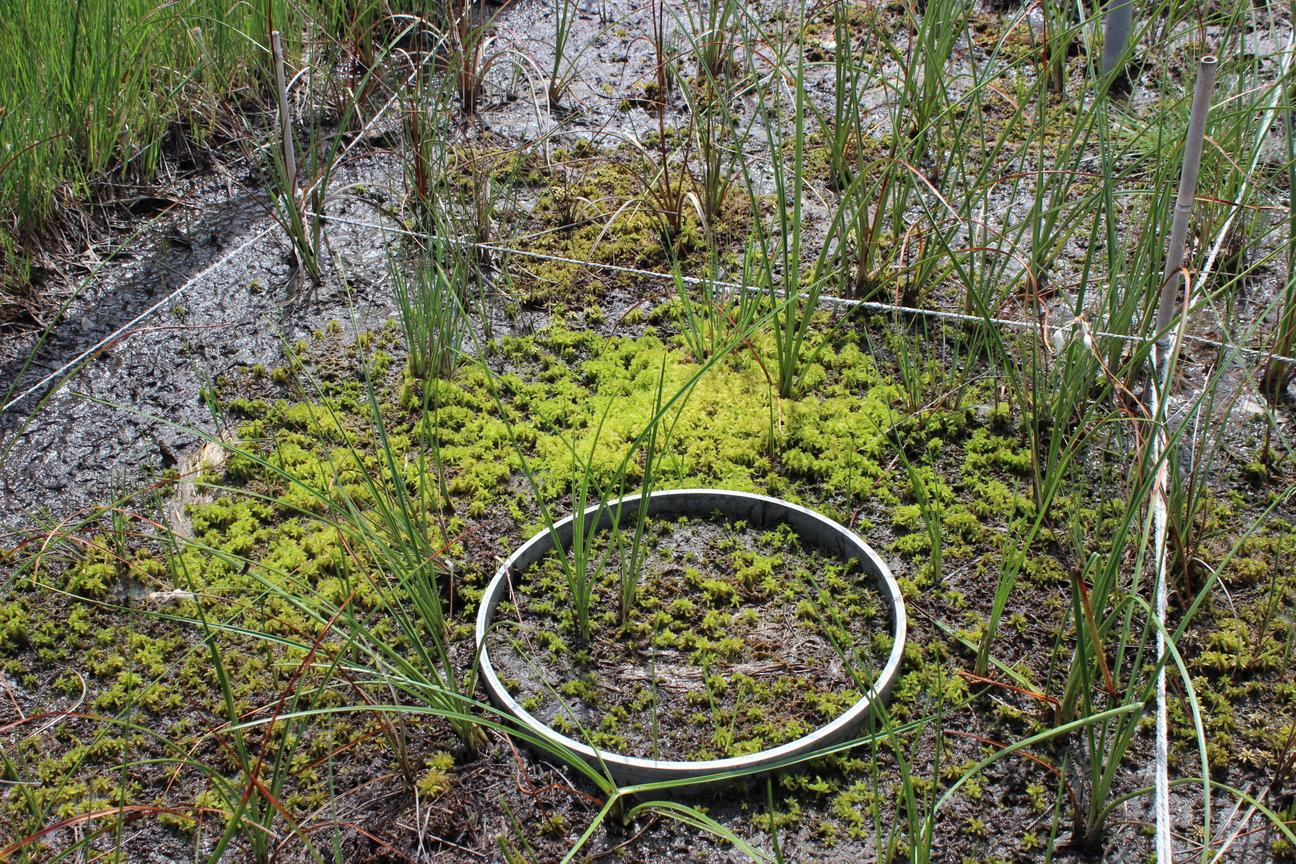
\includegraphics[trim=5cm 0cm 0cm 10cm, clip=true, width=\textwidth]{chap2/sphaigne_eriophorum_c.jpg}
        \caption{\textit{Sphagnum} -- \textit{Eriophorum augustifolium}}\label{fig:sphg_erio}
    \end{subfigure}
    
%    ~ % ce symbole ajoute un espacement horisontal entre les premières deux images
    \begin{subfigure}[b]{0.49\textwidth}
%        \centering 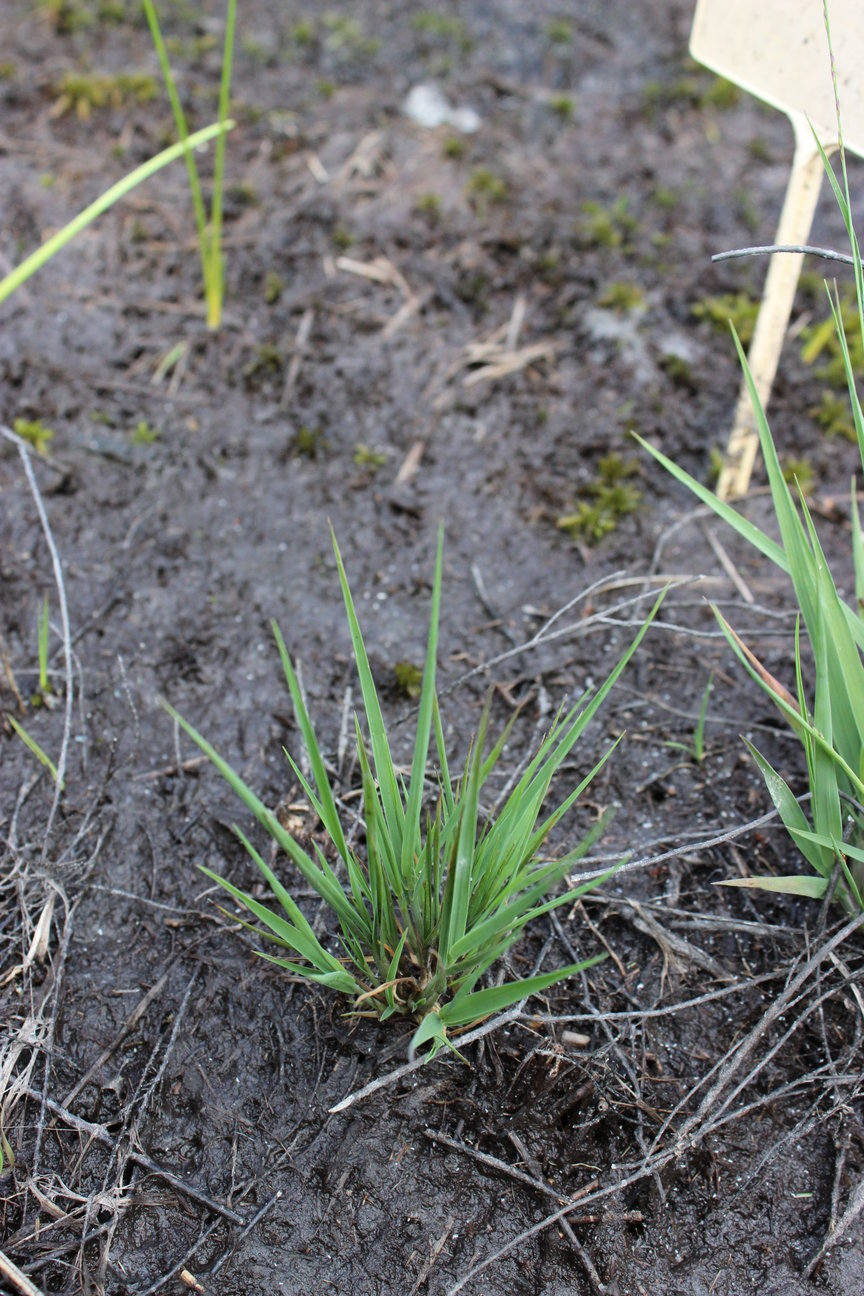
\includegraphics[trim=0cm 0cm 0cm 0cm, clip=true, width=\textwidth]{chap2/molinia_caerulea_c.jpg}
        \centering 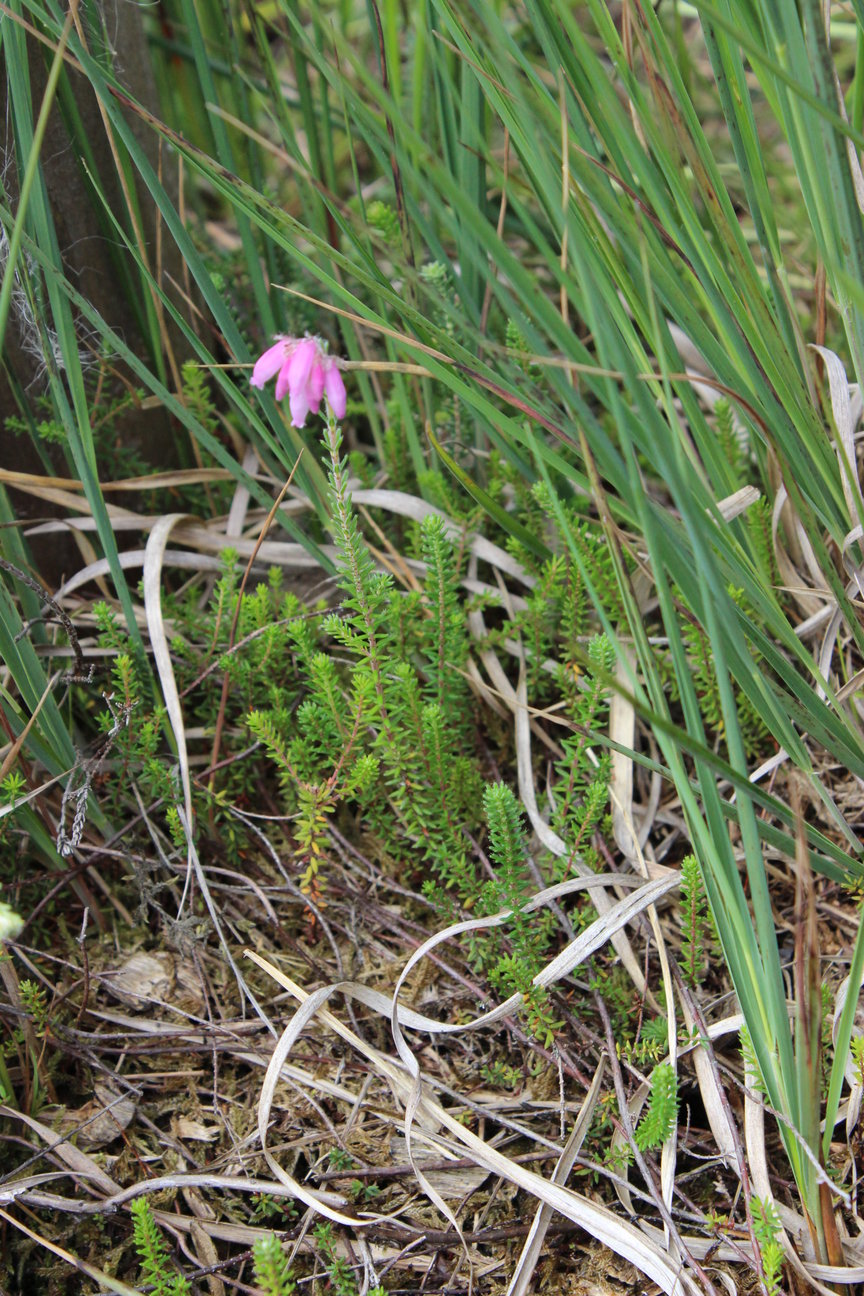
\includegraphics[trim=0cm 4cm 0cm 0cm, clip=true, width=\textwidth]{chap2/erica_tetralix_c.jpg}
        \caption{\textit{Erica tetralix} -- \textit{Molinia caerulea}}\label{fig:erica}
    \end{subfigure}
    % la ligne blanche correspond au retour à la ligne après le deuxième image
    \begin{subfigure}[b]{0.49\textwidth}
        \centering 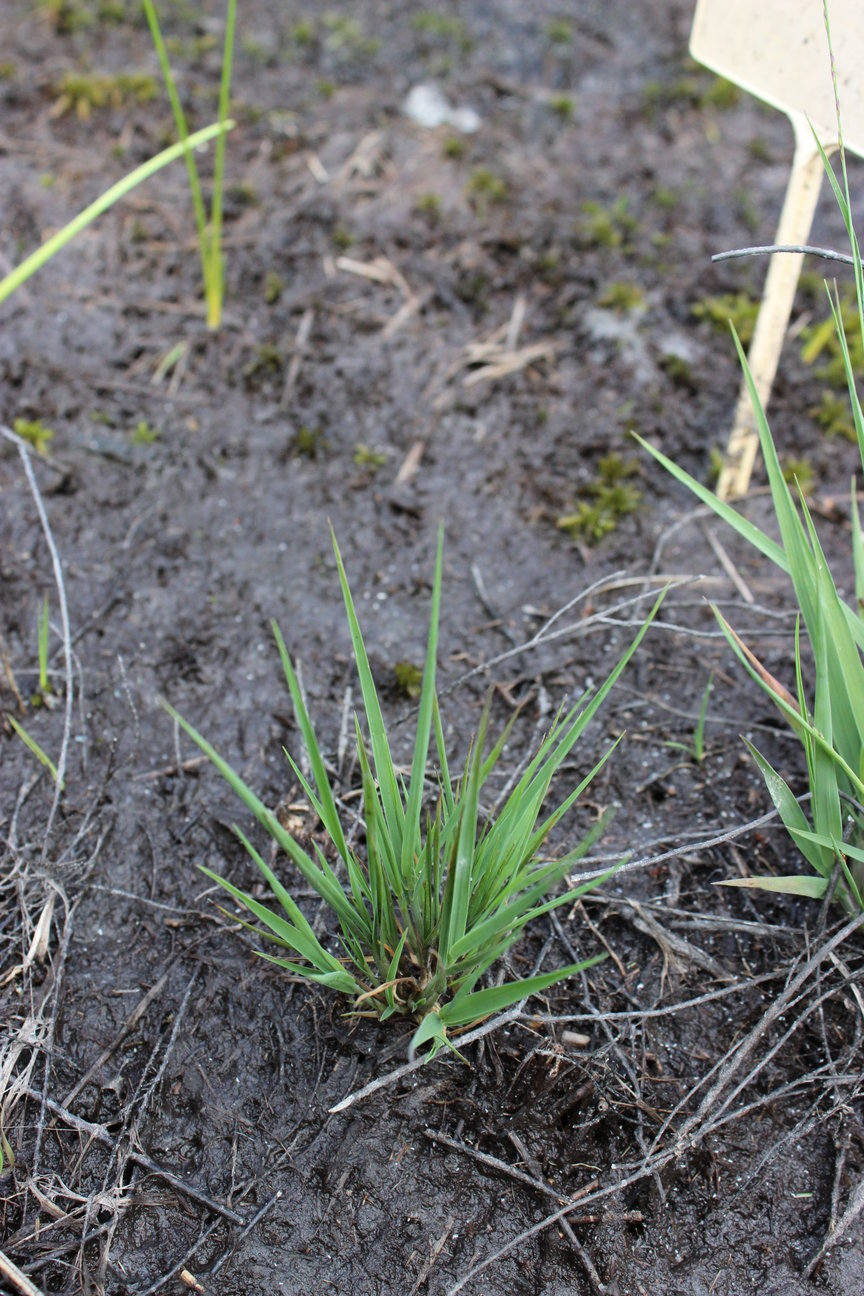
\includegraphics[trim=0cm 2cm 0cm 2cm, clip=true, width=\textwidth]{chap2/molinia_caerulea_c.jpg}
%        \centering 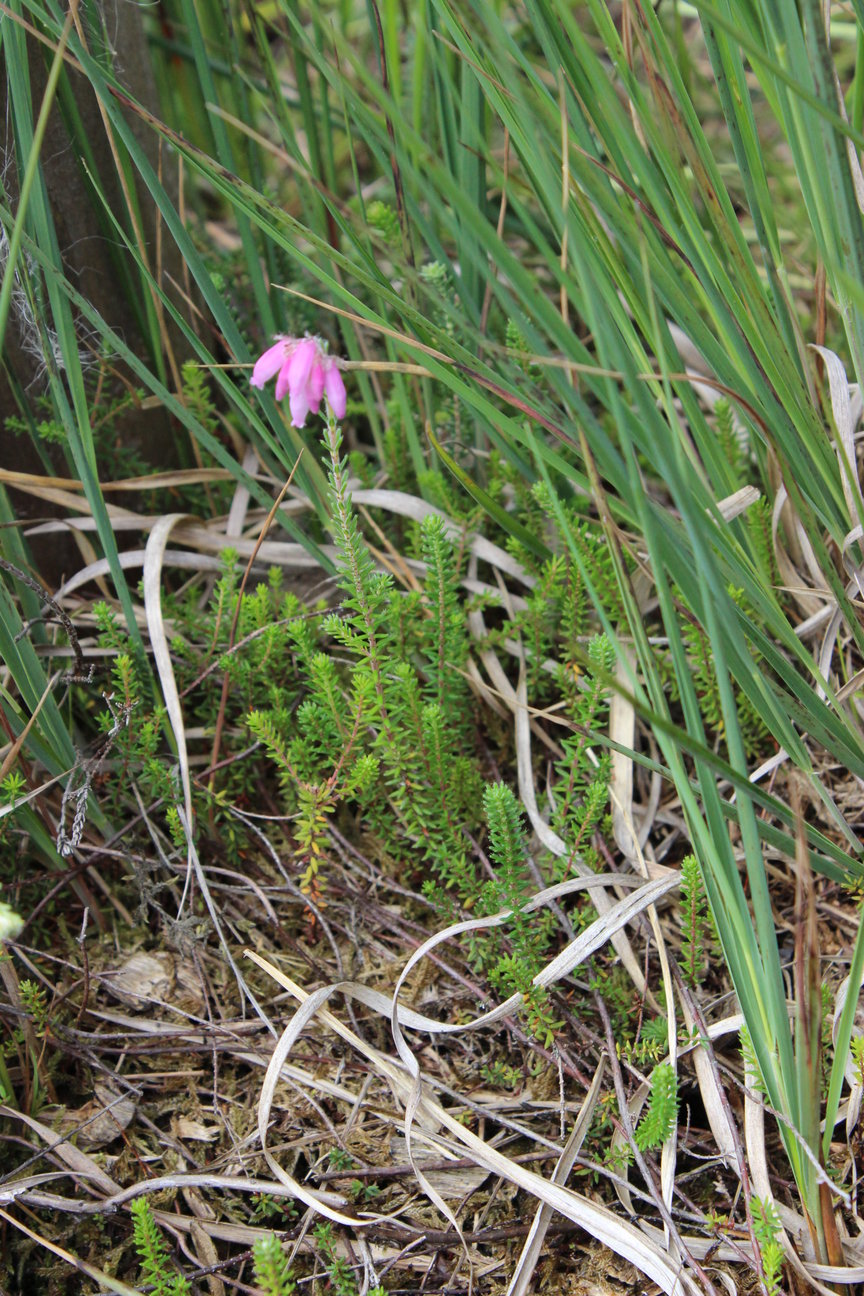
\includegraphics[trim=0cm 0cm 0cm 0cm, clip=true, width=\textwidth]{chap2/erica_tetralix_c.jpg}
        \caption{\textit{Molinia caerulea}}\label{fig:mol}
    \end{subfigure}
%    ~

%    \begin{subfigure}[b]{.8\textwidth}
%        \centering 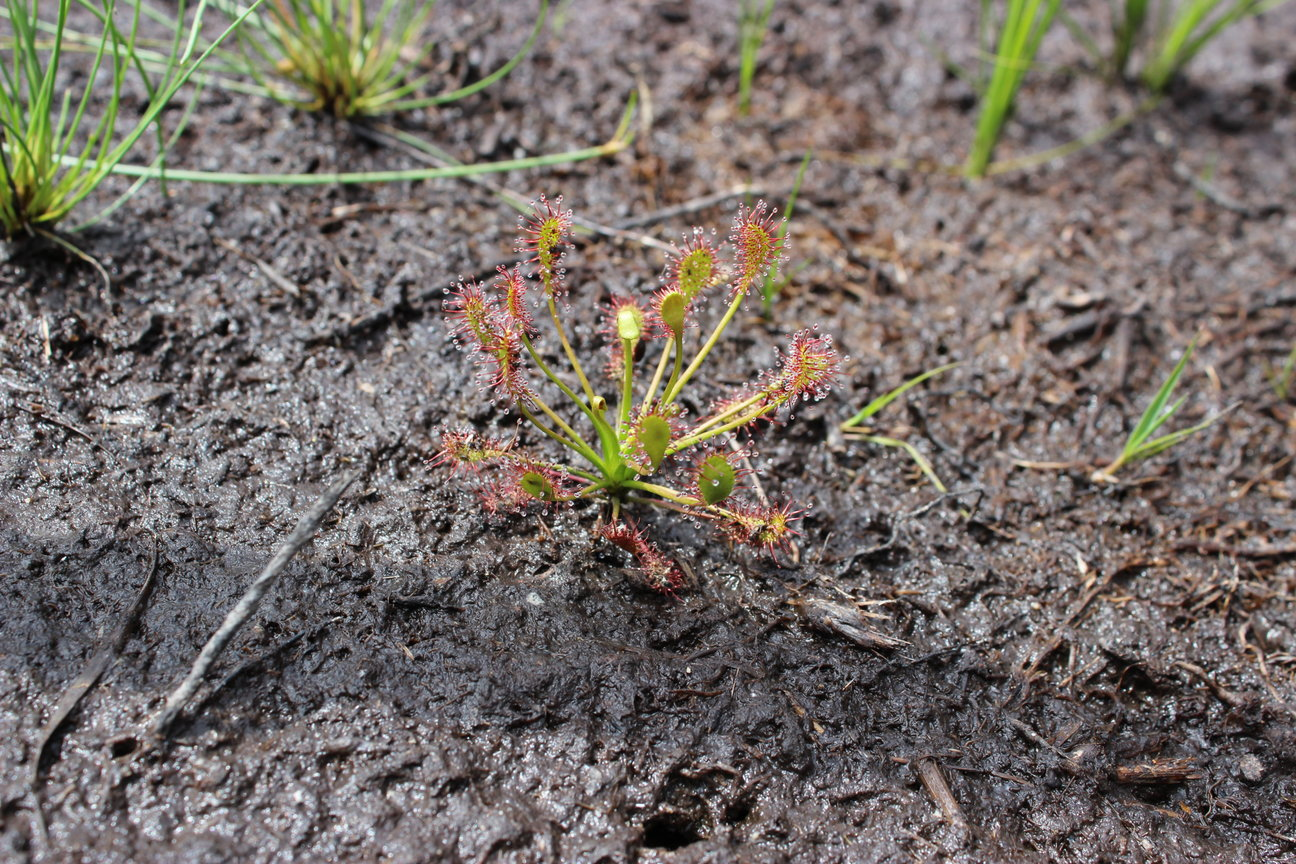
\includegraphics[trim=2.5cm 5cm 2.5cm 5cm, clip=true, width=\textwidth]{chap2/drosera_c.jpg}
%        \caption{drosera}\label{fig:dro}
%    \end{subfigure}
    \caption{Végétation présente sur le site de La Guette, et suivie lors des campagnes de mesure.}\label{fig:veg}
\end{figure}


\begin{figure}
\centering
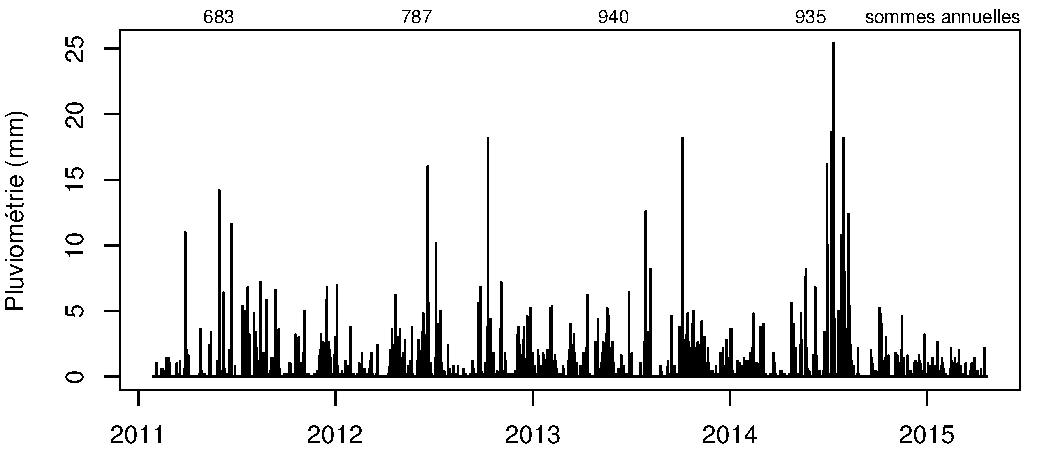
\includegraphics[width=\textwidth]{chap2/pluvio}
\caption{Évolution du niveau de la pluviométrie, en \si{\mm}, des années 2011 à 2014}
\label{fig:pluvio}
\end{figure}

\begin{figure}
\centering
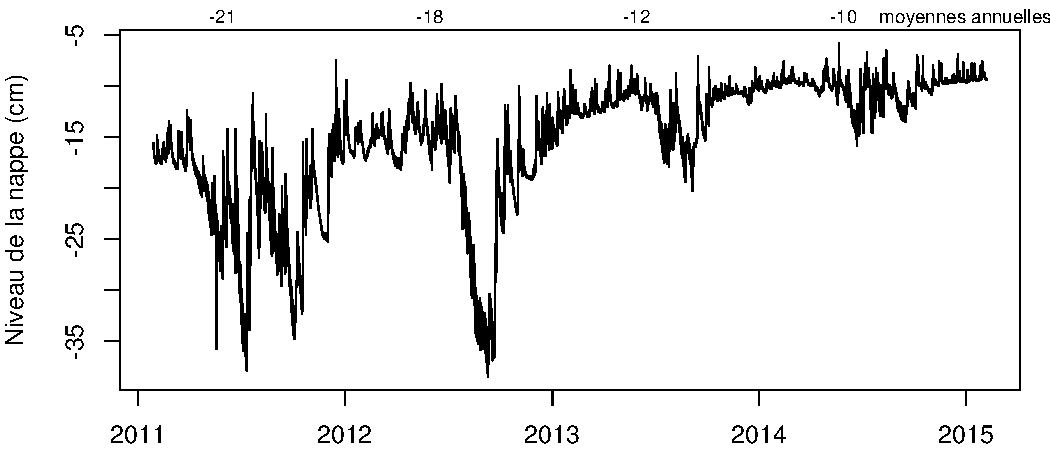
\includegraphics[width=\textwidth]{chap2/WTL}
\caption{Évolution du niveau de la nappe, en cm par rapport à la surface, des années 2011 à 2014}
\label{fig:WTL}
\end{figure}

Au cours des dernières années, les précipitations sont relativement différentes avec deux années plus sèche que la moyenne avant 2013 et deux années plus humide en 2013 et 2014 (Figure~\ref{fig:pluvio}).
On observe également cette dualité au niveau du niveau de la nappe.
Avant 2013 les étés sont marqués par des étiages important avec des baisses du niveau de nappe allant jusqu'à \SI{-60}{\cm} en 2012 (Figure~\ref{fig:WTL}).
Après 2013, les étiages sont beaucoup moins importants sur le site.



\begin{figure}
\centering
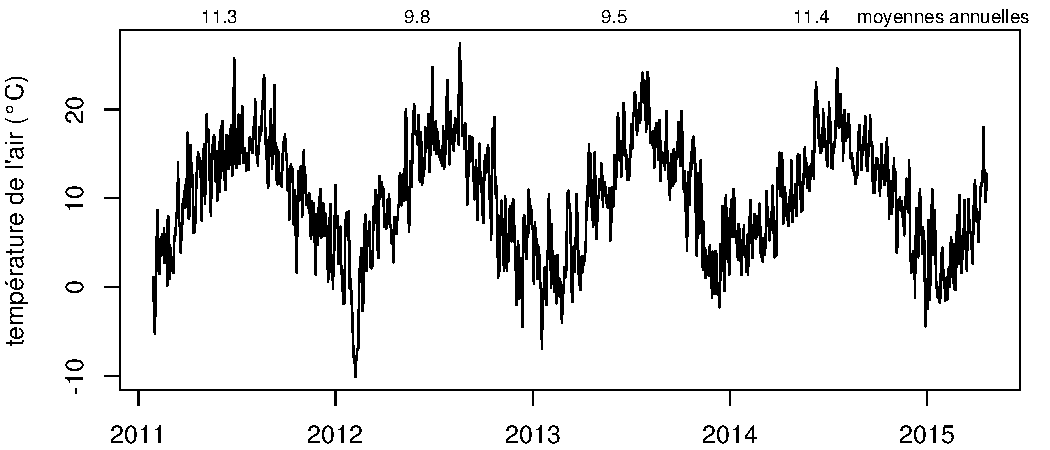
\includegraphics[width=\textwidth]{chap2/tair}
\caption{Évolution de la température de l'air (en \textdegree C) des années 2011 à 2014}
\label{fig:tair}
\end{figure}



Au sein de ses sites de nombreuses mesures ont été effectuée et notamment des mesures de flux de GES à la fois concernant le CO2 et le CH4. La méthodologie étant transverse à de nombreuses expérimentations il convient de l'expliquer au préalable.

\section{Mesures de flux}
\label{sec:clsd_chbr_method}

\subsection{Présentation des méthodologies possibles}
De nombreuses techniques permettent de mesurer des flux de gaz, avec en premier lieu les méthodes de chambres.


Les chambres peuvent être ouvertes, c'est à dire que la mesure se fait lorsque le gaz à l'intérieur de la chambre à l'équilibre avec celui à l'extérieur, ou fermées, dans ce cas le gaz à l'intérieur de la chambre n'est pas à l'équilibre avec celui à l'extérieur.
Elles peuvent également être dynamique, lorsqu'un système de pompe, permettant notamment de transporter le gaz jusqu'à l'analyseur, est présent.
Ou statique si le système est sans flux artificiel.

Trois grandes techniques de chambre existent.
D'abord les chambres \textbf{dynamiques ouvertes} qui se basent sur un état d'équilibre et mesurent une différence de concentration d'un gaz dont une partie passe par la chambre et l'autre non. 
Cette méthode nécessite un système de pompe et donc le passage d'un flux.
Ensuite les chambres \textbf{dynamiques fermées} qui mesurent l'évolution de la concentration du gaz au sein de la chambre à l'aide d'un système de pompe permettant l'envoi du gaz dans un analyseur externe.
Enfin les chambres \textbf{statiques fermées} qui mesurent également l'évolution de la concentration du gaz au sein de la chambre sans qu'un système de pompe ne soit présent.
Dans ce cas soit l'analyseur est présent dans la chambre, soit des prélèvements sont fait à intervalles réguliers puis analysés par la suite en chromatographie gazeuse.

Il faut noter que les dénominations anglaises de ces méthodes doit faire l'objet d'une attention particulière.
\textit{Closed chamber} par exemple est parfois utilisé pour se référer à l'état ou non d'équilibre, comme défini dans ce document, mais parfois également pour désigner les méthodes de chambre sans système de flux ce qui peut prêter à confusion \cite{pumpanen2004}.
Souvent utilisées les dénominations \textit{open}/\textit{closed} et \textit{dynamic}/\textit{static} sont décrites dans \cite{luo2006161}, une autre convention peut être rencontrée : \textit{flow-through}/\textit{non-flow-through} et \textit{steady state}/\textit{non-steady state} \cite{livingston1995}

Ces différentes méthodes ont divers avantages et inconvénients.

Ces méthodes sont souvent utilisées car elles on un coût modeste, et sont très versatiles ce qui permet leur utilisation dans de nombreuses situations.
D'autres méthodes plus globales existent comme les méthodes d'Eddy Covariance.

Les méthodes d'Eddy Covariance se base sur...

Comparaison entre les méthodes de chambre et les méthodes d'Eddy Covariance.

\subsection{Les mesures de \coo}

Toutes les mesures de \coo présentées par la suite ont été faite avec les mêmes matériels et le même protocole.
Les chambres en \textbf{XXXX} ont été conçue (LPC2E) fabriquées (ISTO) au CNRS.
Ce sont des chambres transparentes, cylindrique, de \SI{30}{\centi\metre} de diamètre et \SI{30}{\centi\metre} de hauteur.
Les mesures de \coo à proprement parler ont été faite à l'aide d'une sonde Vaisala GMP 343\textregistered.
La sonde est directement inséré dans la chambre ainsi qu'une sonde Vaisala \textbf{XXXXX} mesurant d'humidité et la température dans la chambre.

Avant toute mesure, des embases sont installées sur le site.
Ce sont des cylindres de PVC d'une hauteur de \SI{15}{\centi\metre} inséré dans le sol sur 8 à \SI{10}{\centi\metre}.
La partie enterrée de ces cylindres ayant préalablement été percée d'une quarantaine de trou afin de minimiser les impacts de l'embase sur le développement racinaire et les écoulements d'eau.

La méthode mise en œuvre est celle de la chambre statique fermée.
Aucun système de pompe n'est donc utilisé, la chambre est posée sur l'embase, elle contient l'analyseur de \coo qui mesure la variation de la concentration en gaz au cours du temps.
Un ventilateur de faible puissance est également présent à l'intérieur de la chambre afin d'homogénéiser l'air présent dans la chambre.
1 à \SI{3}{\minute} sont nécessaires après la pose de la chambre afin d'éviter les effets pouvant y être liés.
Ensuite l’enregistrement est lancé, avec l'acquisition toutes les \SI{5}{\second} pendant \SI{5}{\minute} de la concentration en \coo, de la température et de l'humidité.
La mesure se déroule donc sur une période de temps relativement courte afin de minimiser le déséquilibre avec le milieu extérieur.
Dans ce but les mesures on parfois été encore raccourcie, 2 à \SI{3}{\minute} d'acquisition, si une pente claire se dégage rapidement, notamment lorsque les conditions météorologiques, chaudes et ensoleillées, laissaient supposer une différence importante vis à vis des conditions extérieures.

Généralement, deux acquisitions de \coo sont faites à la suite sur une embase.
La première, avec la chambre transparente nue, permettant l'enregistrement de l'ENE (Figure~\ref{fig:chb}-a).
La seconde avec la chambre recouverte d'une chaussette de tissu occultant, isolant la chambre de la lumière, permettant d'interrompre la photosynthèse et donc d'enregistrer les respirations (RE) (Figure~\ref{fig:chb}-b).

\begin{figure}
	\centering
	\begin{subfigure}[t]{0.5\textwidth}
		\centering
		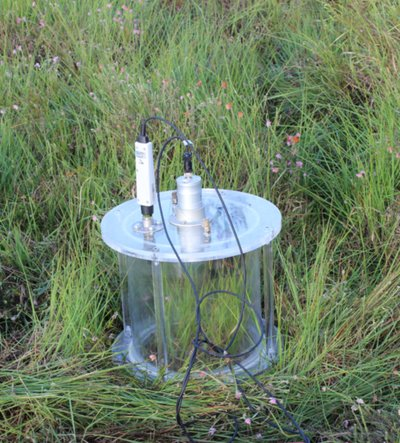
\includegraphics[width=.8\textwidth, frame]{chap2/chb_ENE}
	\end{subfigure}%
	\begin{subfigure}[t]{0.5\textwidth}
		\centering
		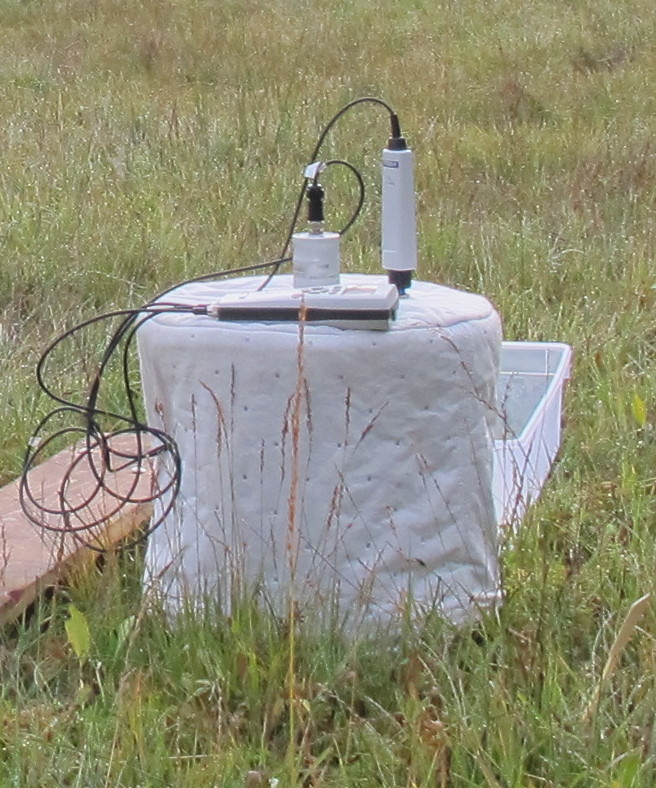
\includegraphics[width=.8\textwidth, frame]{chap2/chb_ER}
	\end{subfigure}%

	\begin{subfigure}[t]{0.5\textwidth}
		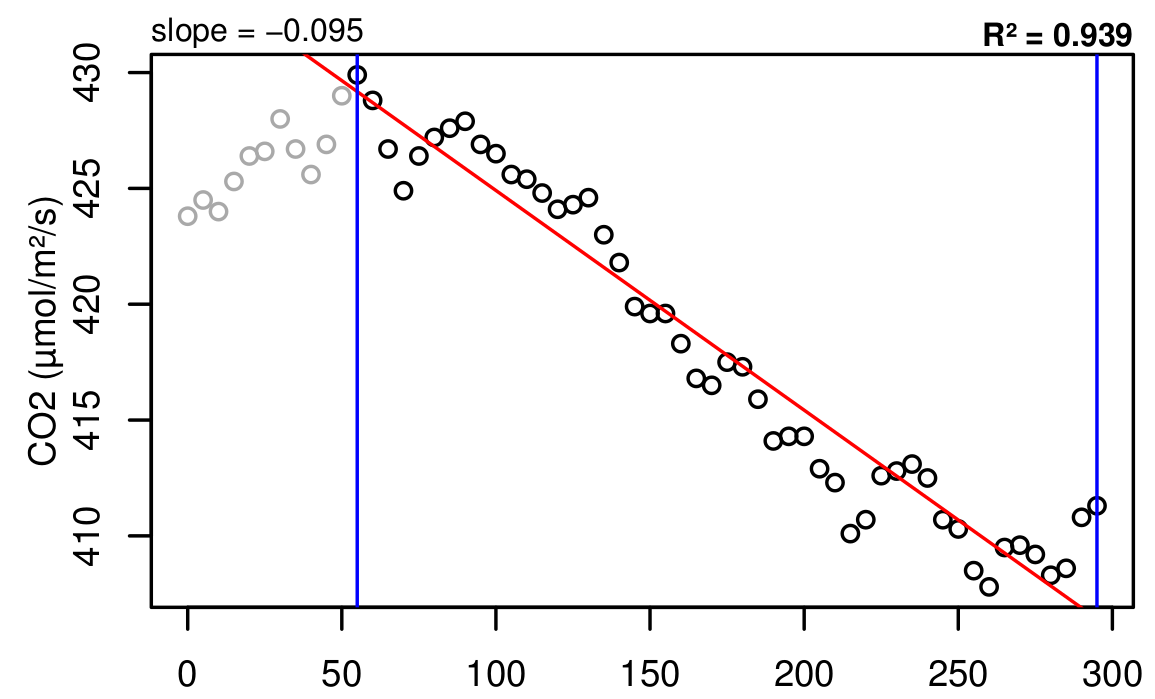
\includegraphics[width=\textwidth]{chap2/chb_ENE_reg}
		\caption{Mesure de l'échange net de l'écosystème}
	\end{subfigure}%
	\begin{subfigure}[t]{0.5\textwidth}
		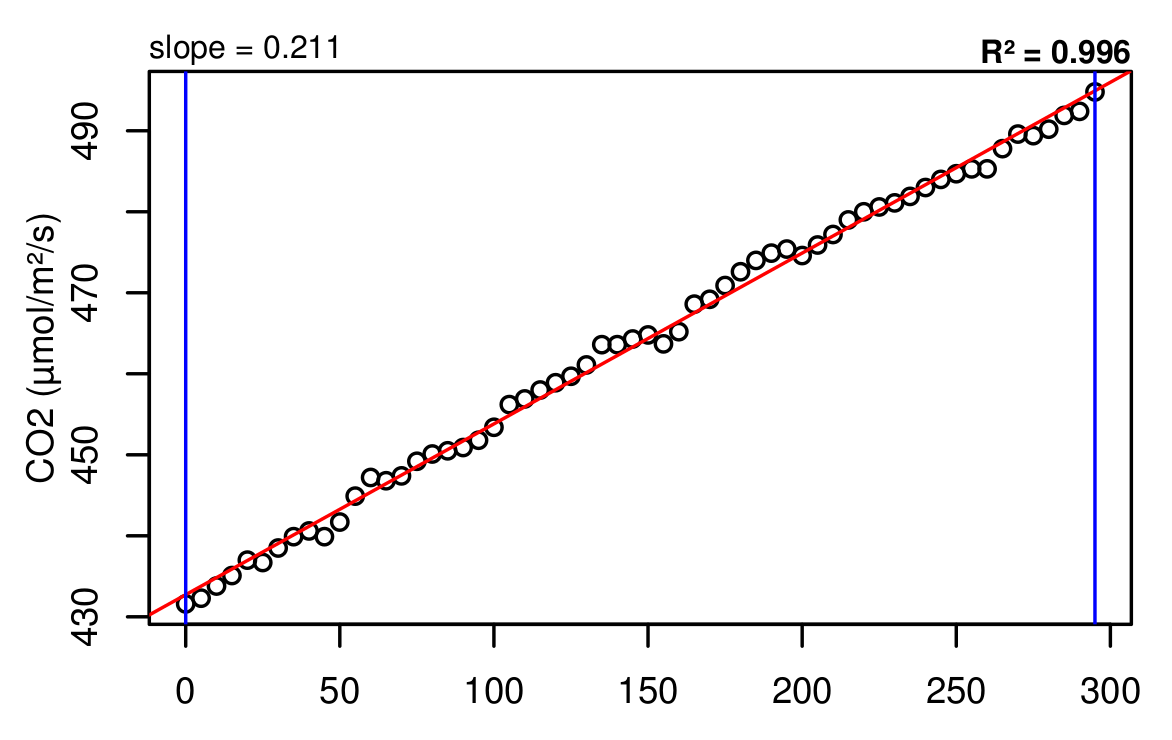
\includegraphics[width=\textwidth]{chap2/chb_ER_reg}
		\caption{Mesure de la respiration de l'écosystème}
	\end{subfigure}
%    \caption{Caption place holder}
\caption{Mesures de \coo}
\label{fig:chb}
\end{figure}


De nombreux écueils peuvent rendre une mesure inexploitable. D'abord le placement de la chambre, cela peut sembler trivial mais positionner la chambre au milieu d'herbacées et de bruyère n'est pas toujours évident. Plus anecdotiquement des sphaignes gelées, recouvrant les bords de l'embase rendent la pose de la chambre difficile voire impossible. Selon l'heure de la journée des gradients de concentrations peuvent être présent et augmenter localement les concentrations de CO2 de façon importante allant jusqu'à saturer la sonde.

Au vu du volume de données acquises et souhaitant garder l'intérêt de mesure manuelle, à savoir le contrôle humain des flux et des conditions de mesure, il a été nécessaire de développer un outil de traitement facilitant le contrôle et le calcul des flux.
Ceci afin d'éviter de recourir à des seuils arbitraires (typiquement une valeur de R$^{2}$) pour le contrôle qualité des données, mais également de permettre une reproductibilité et un traçage des modifications effectuées sur les données brutes.
(donner des exemples)

\subsection{Les mesures de \chh}

\begin{figure}
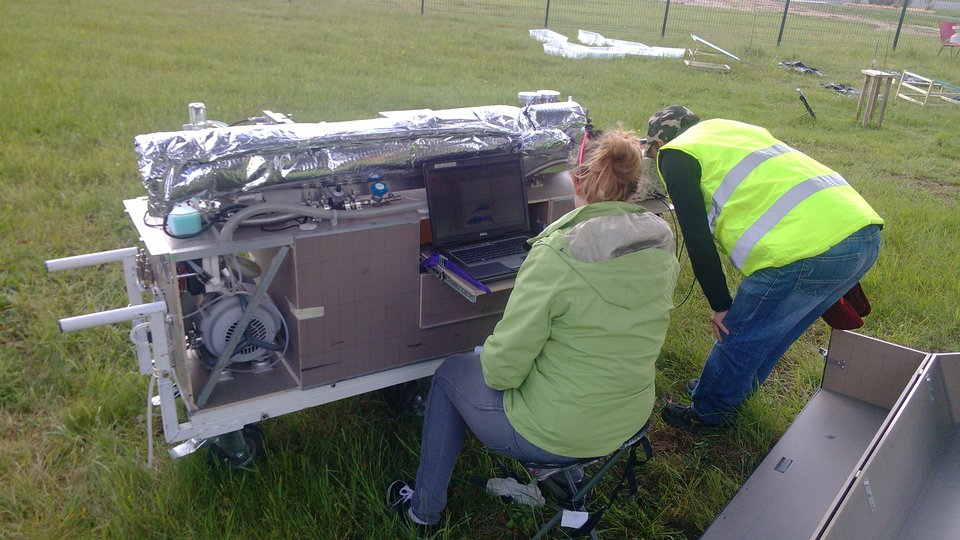
\includegraphics[width=\textwidth]{chap2/SPIRIT_terrain}
\caption{SPIRIT}
\label{fig:SPIRIT}
\end{figure}

Les mesures de \chh ont été réalisée avec une chambre aux caractéristiques similaires à celles utilisées pour les mesures de \coo à l'exception de l'interface avec l'analyseur.
La méthode de la chambre dynamique fermée a été utilisée pour réaliser ces mesures, elle diffère donc légèrement de celle utilisée pour le \coo puisqu'elle nécessite la mise en oeuvre d'un système de pompe pour transporter le gaz jusqu'à l'analyseur.
Les mesures de concentration en \chh ont été réalisée à l'aide d'un instrument développé par le LPC2E, le SPIRIT (Figure~\ref{fig:SPIRIT}).
C'est un SPectrometre Infra Rouge In-situ Troposphérique (son premier objectif étant d'être emporté lors de campagne avion ou ballon ? pour mesurer le \chh de la troposphère.).
Il permet la mesure du \chh à haute fréquence.
Le fonctionnement détaillé de l'appareil est décrit dans \cite{guimbaud2011}.

\begin{equation}
F = \frac{dX}{dt} \times \frac{P}{R \times T} \times \frac{V}{S}
\end{equation}

%QUESTIONS :
%
%*Taille des embases ? Effets de bord ?
%*Perturbation du milieu ? (Mesure de végétation, pose de la chambre, mesure pièzo...)
%*Impact de la strate arborée ?
%*Validité des profils de température ?
%Méthode de Chambre fermée (Biais ?)
%
%Améliorations ? (Lister les amélioration à faire ou non)


\section{Facteurs contrôlants}
Afin de déterminer l'impact de facteurs contrôlants sur ces flux, mesurer les flux ne suffit pas il faut également mesurer les variables environnementales dont on pense qu'elles seront des facteurs contrôlants important.
La description des techniques et matériels communs aux différentes expérimentations utilisées est développée ci-dessous.
Par contre leur mise en œuvre ou caractéristiques spécifiques, comme la fréquence des mesures, sera décrite individuellement au niveau des parties détaillant chacune des expérimentations.

\subsection{acquisitions automatisées}

Les paramètres météorologiques ont été mesurés, en un point, au centre de la tourbière (Figure~\ref{fig:carte_LG})(\textbf{carte ?}) à l'aide d'une station d'acquisition Campbell installée sur le site en 2008.
Les variables ont été acquises à une fréquence horaire jusqu'au 20 février 2014 puis toutes les demi-heures par la suite. 
Les paramètres enregistrés sont la pression atmosphérique, l'humidité relative de l'air, la pluviométrie, l'irradiation solaire, la vitesse et la direction du vent. (\textbf{détail du matos ?}).
Cette même station à également permis l'acquisition de la température de l'air et de la tourbe à \num{-5}, \num{-10}, \num{-20} et \SIlist{-40}{\cm}.
Installées à la même époque, quatre sondes \textbf{OTT ?} de mesure du niveau de la nappe d'eau permettent le suivi du niveau de la nappe dans la tourbière.

\subsection{Protocole d'estimation de la végétation}

Le suivi non-destructif d'une végétation n'est pas triviale et nécessite la mise en place de protocoles particuliers en fonction du type de végétation.
L'objectif est de pouvoir estimer une biomasse produite en impactant au minimum la végétation en place.
Pour l'ensemble des espèces végétales présentes dans les embases servant à la mesure des flux un recouvrement à été estimé, à l’œil.


\subsubsection{La strate arbustive}
Pour la strate arbustive des mesures de hauteur moyenne ont été effectuées, en mesurant depuis le niveau du sol, ou le toit des sphaignes, si elles étaient présentes, jusqu'au sommet de l'individu.
\begin{figure}
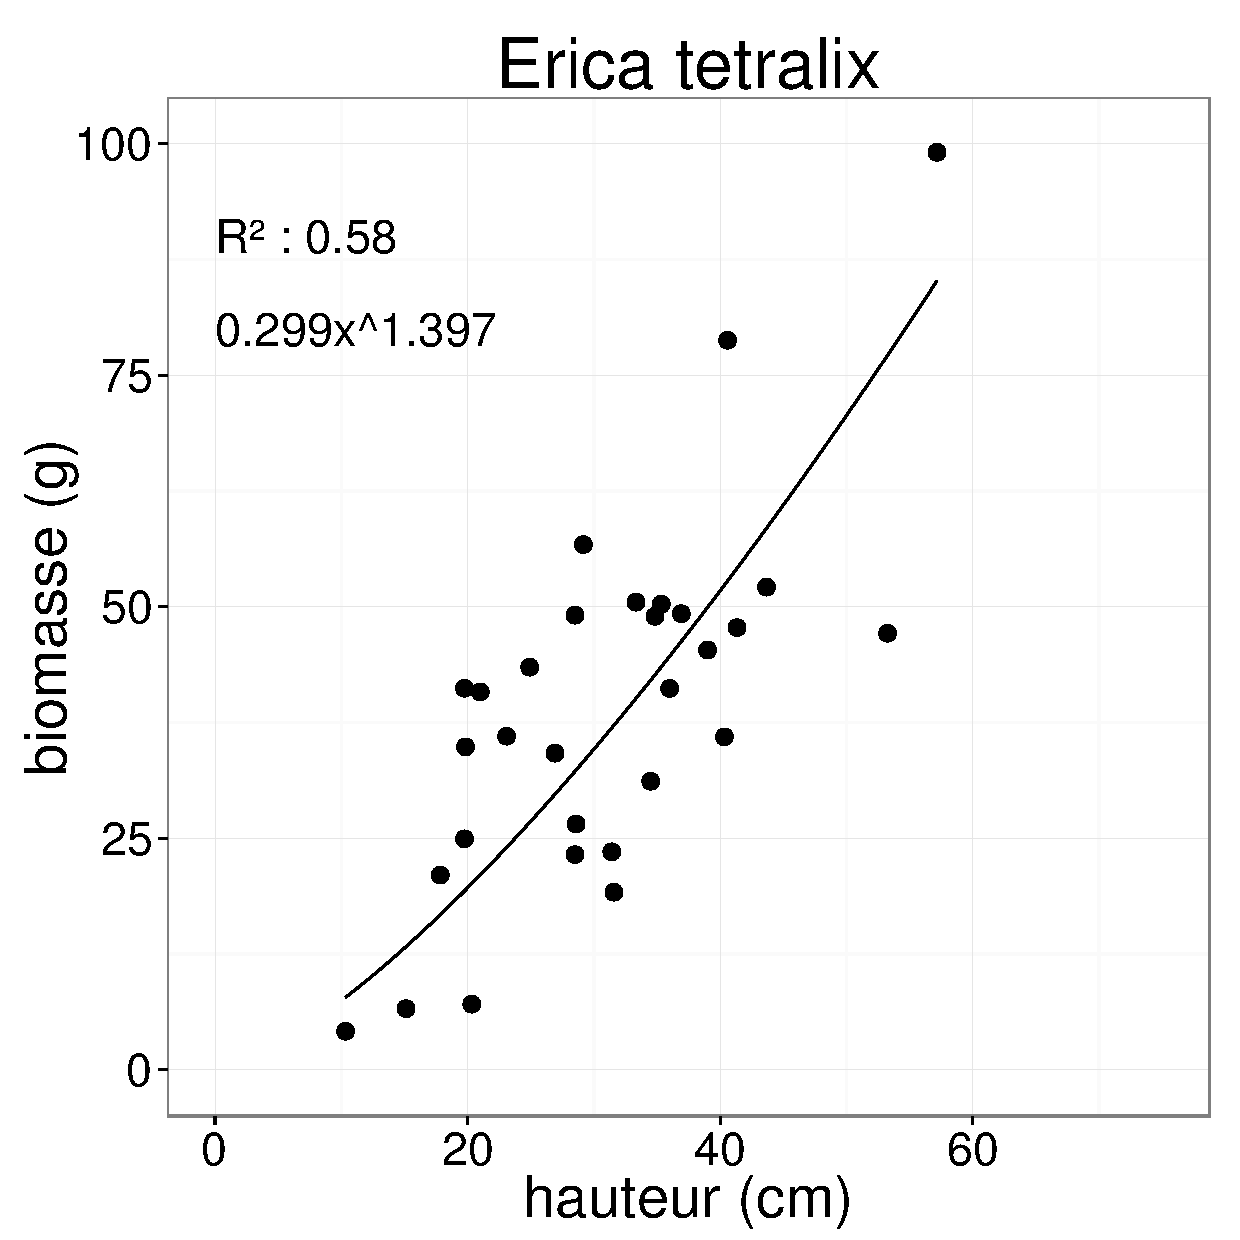
\includegraphics[width=.5\textwidth]{chap2/cal_tetra_eq}
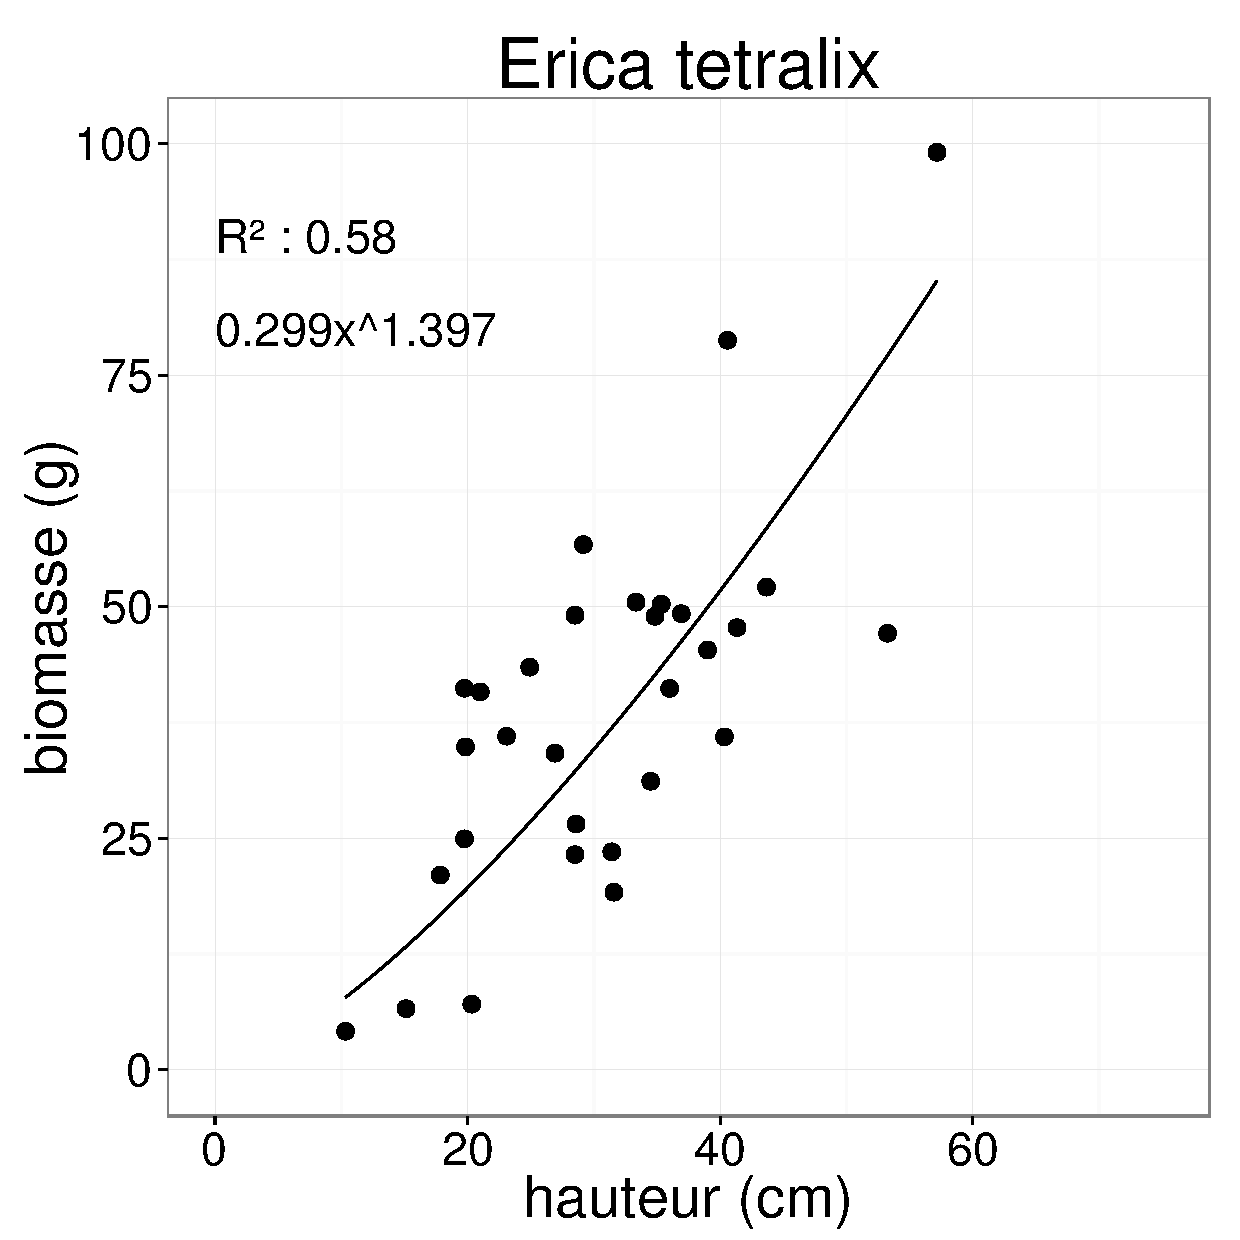
\includegraphics[width=.5\textwidth]{chap2/cal_tetra_eq}
\caption{Calibration de la biomasse en fonction de la hauteur}
\label{fig:cal_arbu}
\end{figure}

\subsubsection{La strate herbacée}
Pour la strate herbacée, en 2013, 5 individus des deux espèces majoritaires (Eriophorum vaginatum ? augustifolium ?, Molinia Caerulea) ont été marqués afin de pourvoir les mesurer plusieurs fois au cours de la saison.
Cependant les difficultés à retrouver les individus marqués couplés à la mort d'un nombre important d'entre eux n'ont pas permis d'acquérir de résultats significatifs.
En conséquence en 2014 ces deux espèces ont fait l'objet de comptage exhaustif et de mesure de hauteur moyenne.


\begin{figure}
	\centering
	\begin{subfigure}[t]{0.5\textwidth}
		\centering
		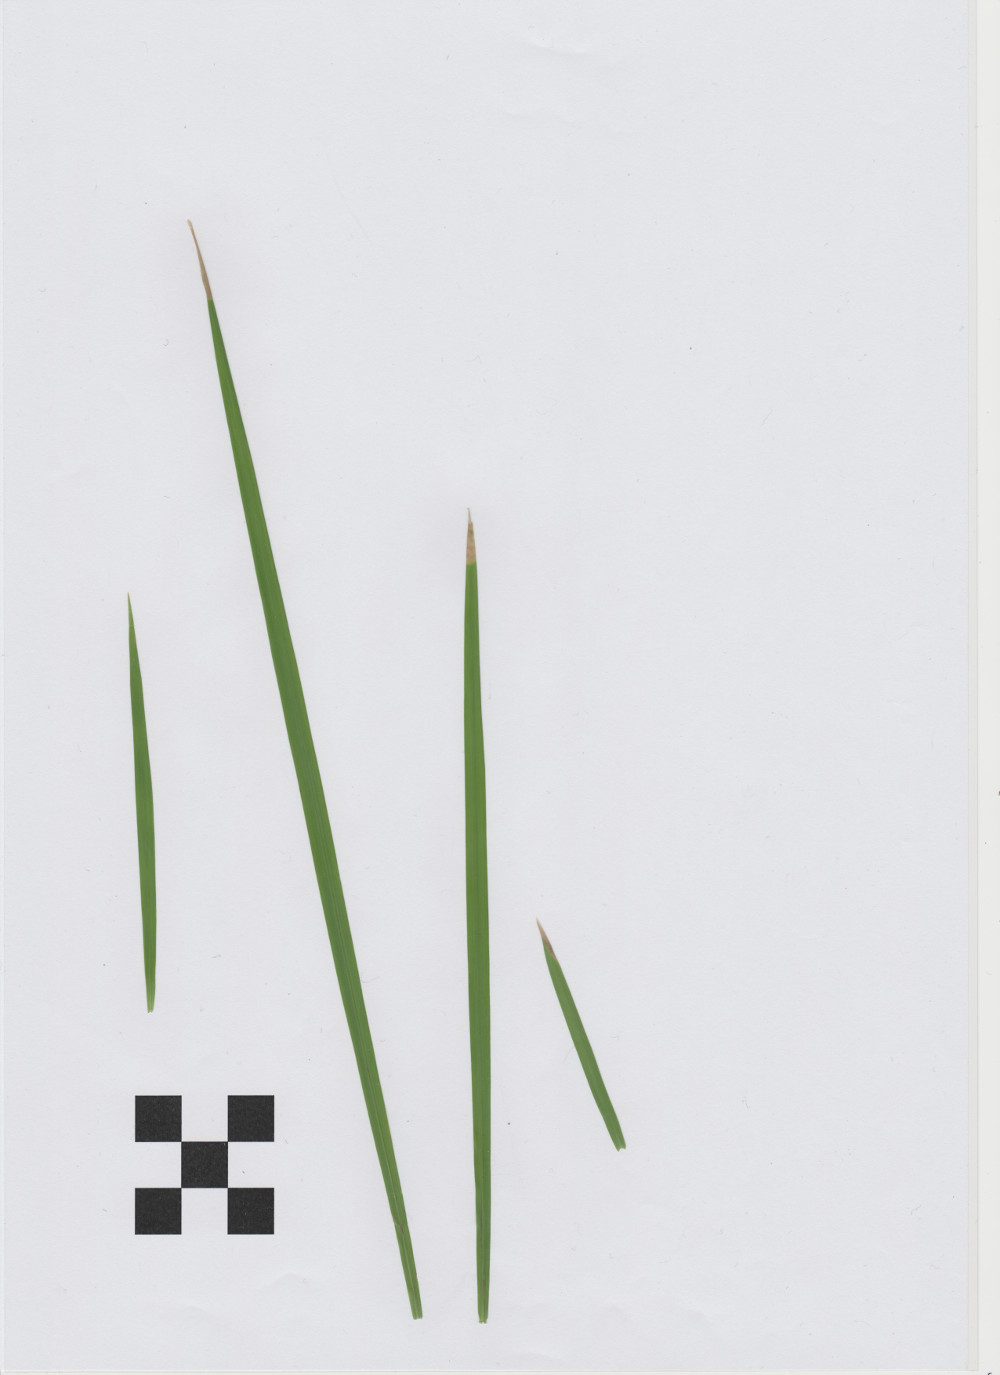
\includegraphics[width=.8\textwidth, frame]{chap2/Cch_moli_A_1to4}
		\caption{image scannée}
	\end{subfigure}%
	\begin{subfigure}[t]{0.5\textwidth}
		\centering
		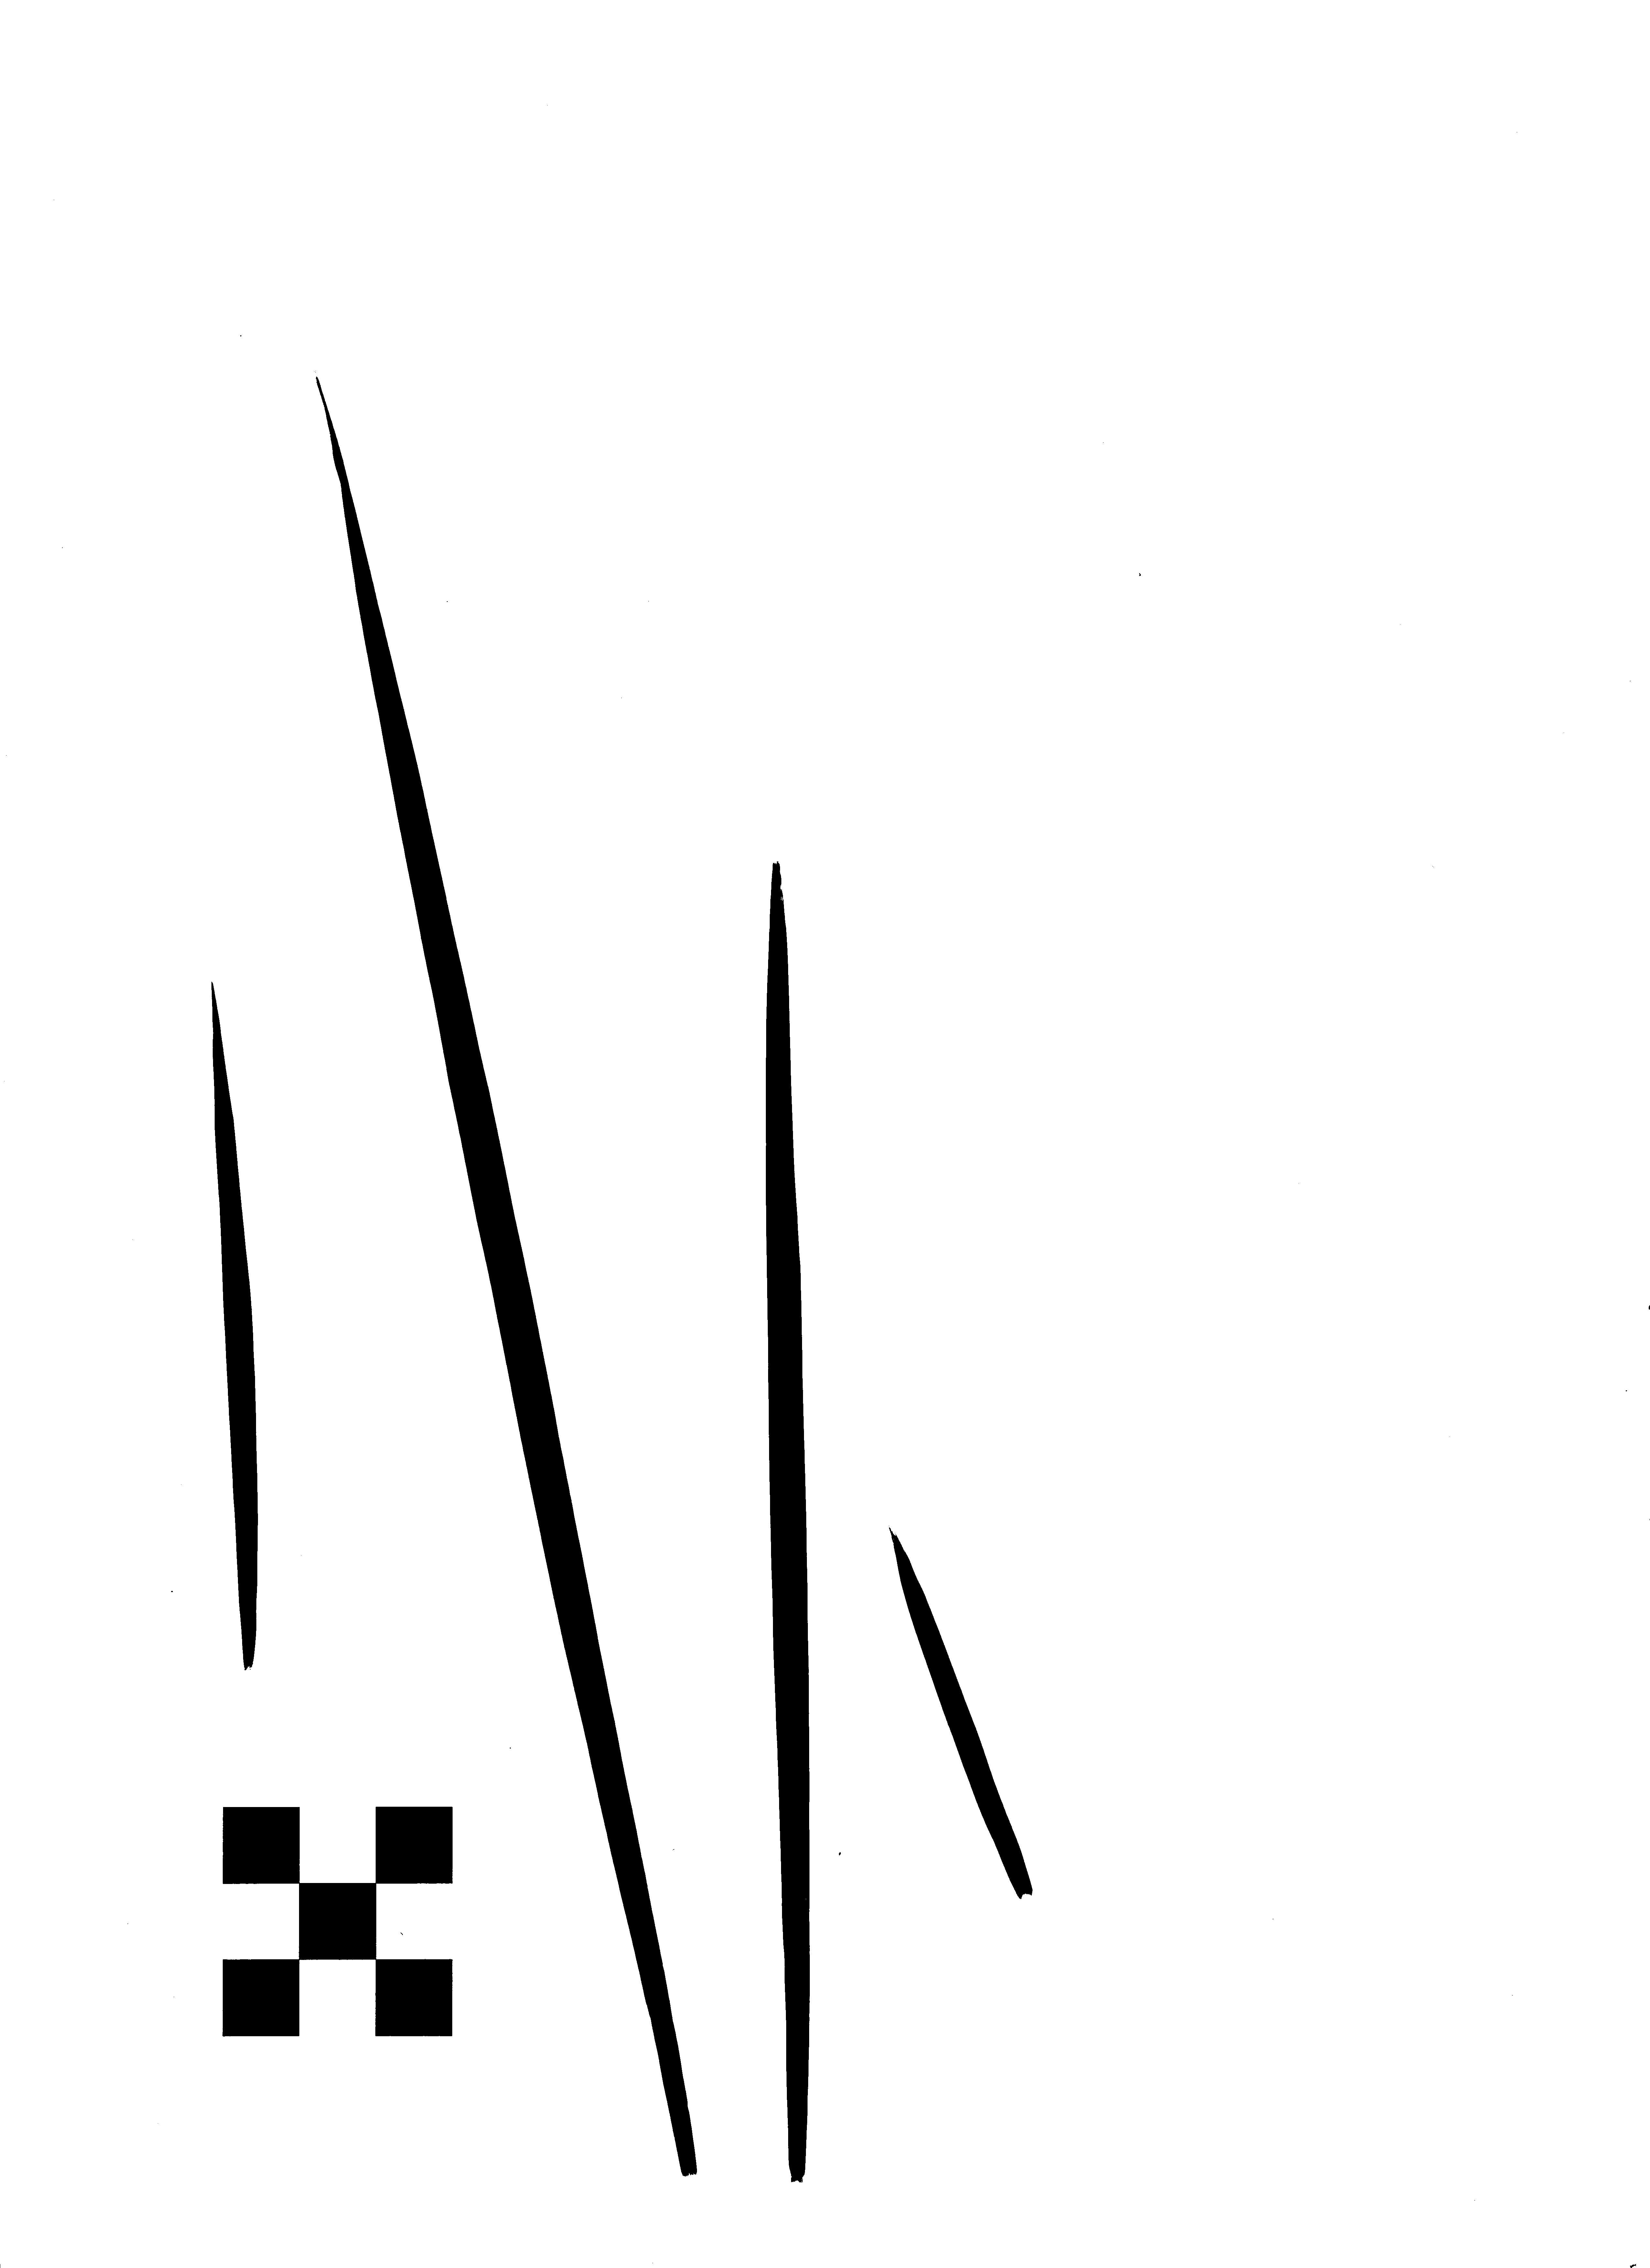
\includegraphics[width=.8\textwidth, frame]{chap2/Cch_moli_A_1to4_mod}
		\caption{image binarisée}
	\end{subfigure}
%    \caption{Caption place holder}
\caption{Scanne des feuilles}
\label{fig:scan_mol}
\end{figure}


\begin{figure}
	\centering
	\begin{subfigure}[t]{0.5\textwidth}
		\centering
		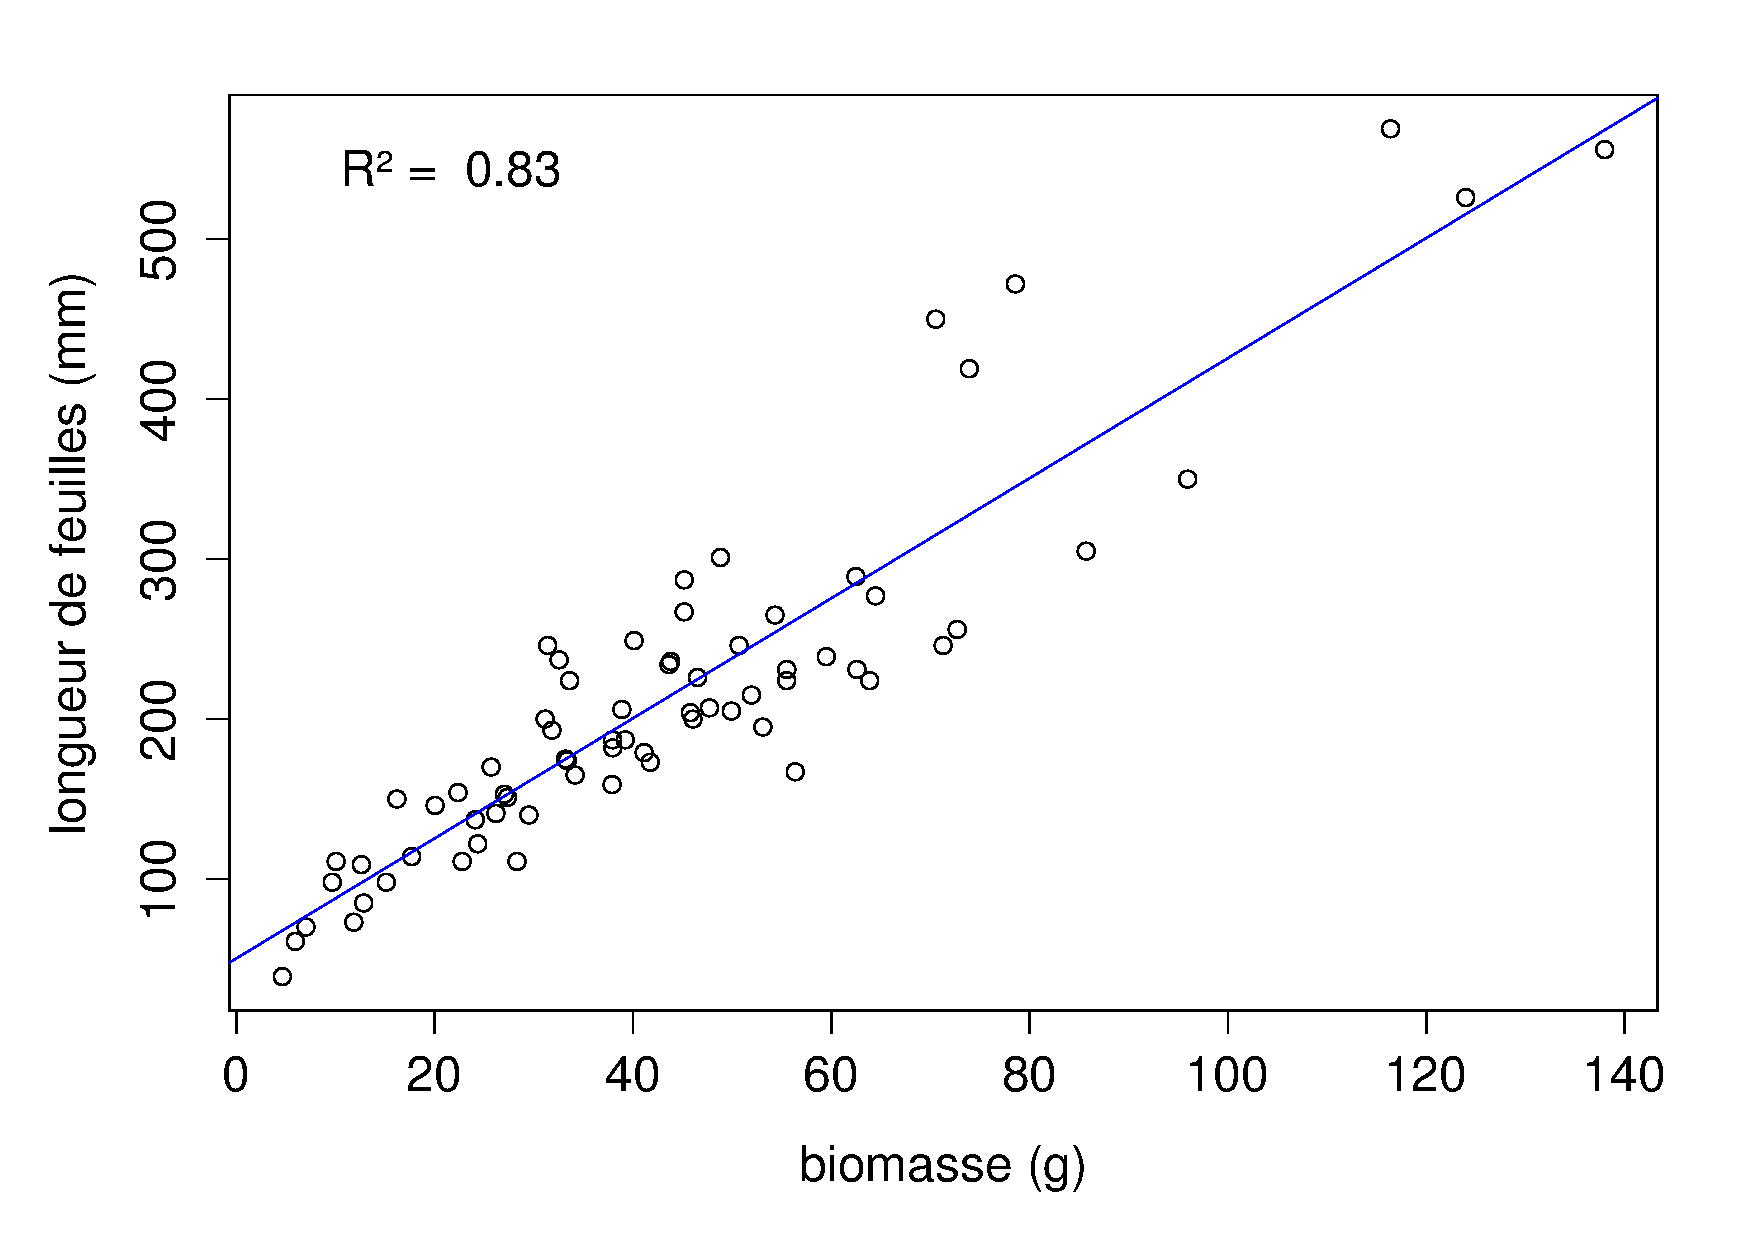
\includegraphics[width=\textwidth]{chap2/mol_lon_bioM}
		\caption{Molinia caerulea -- biomasse}
	\end{subfigure}%
	\begin{subfigure}[t]{0.5\textwidth}
		\centering
		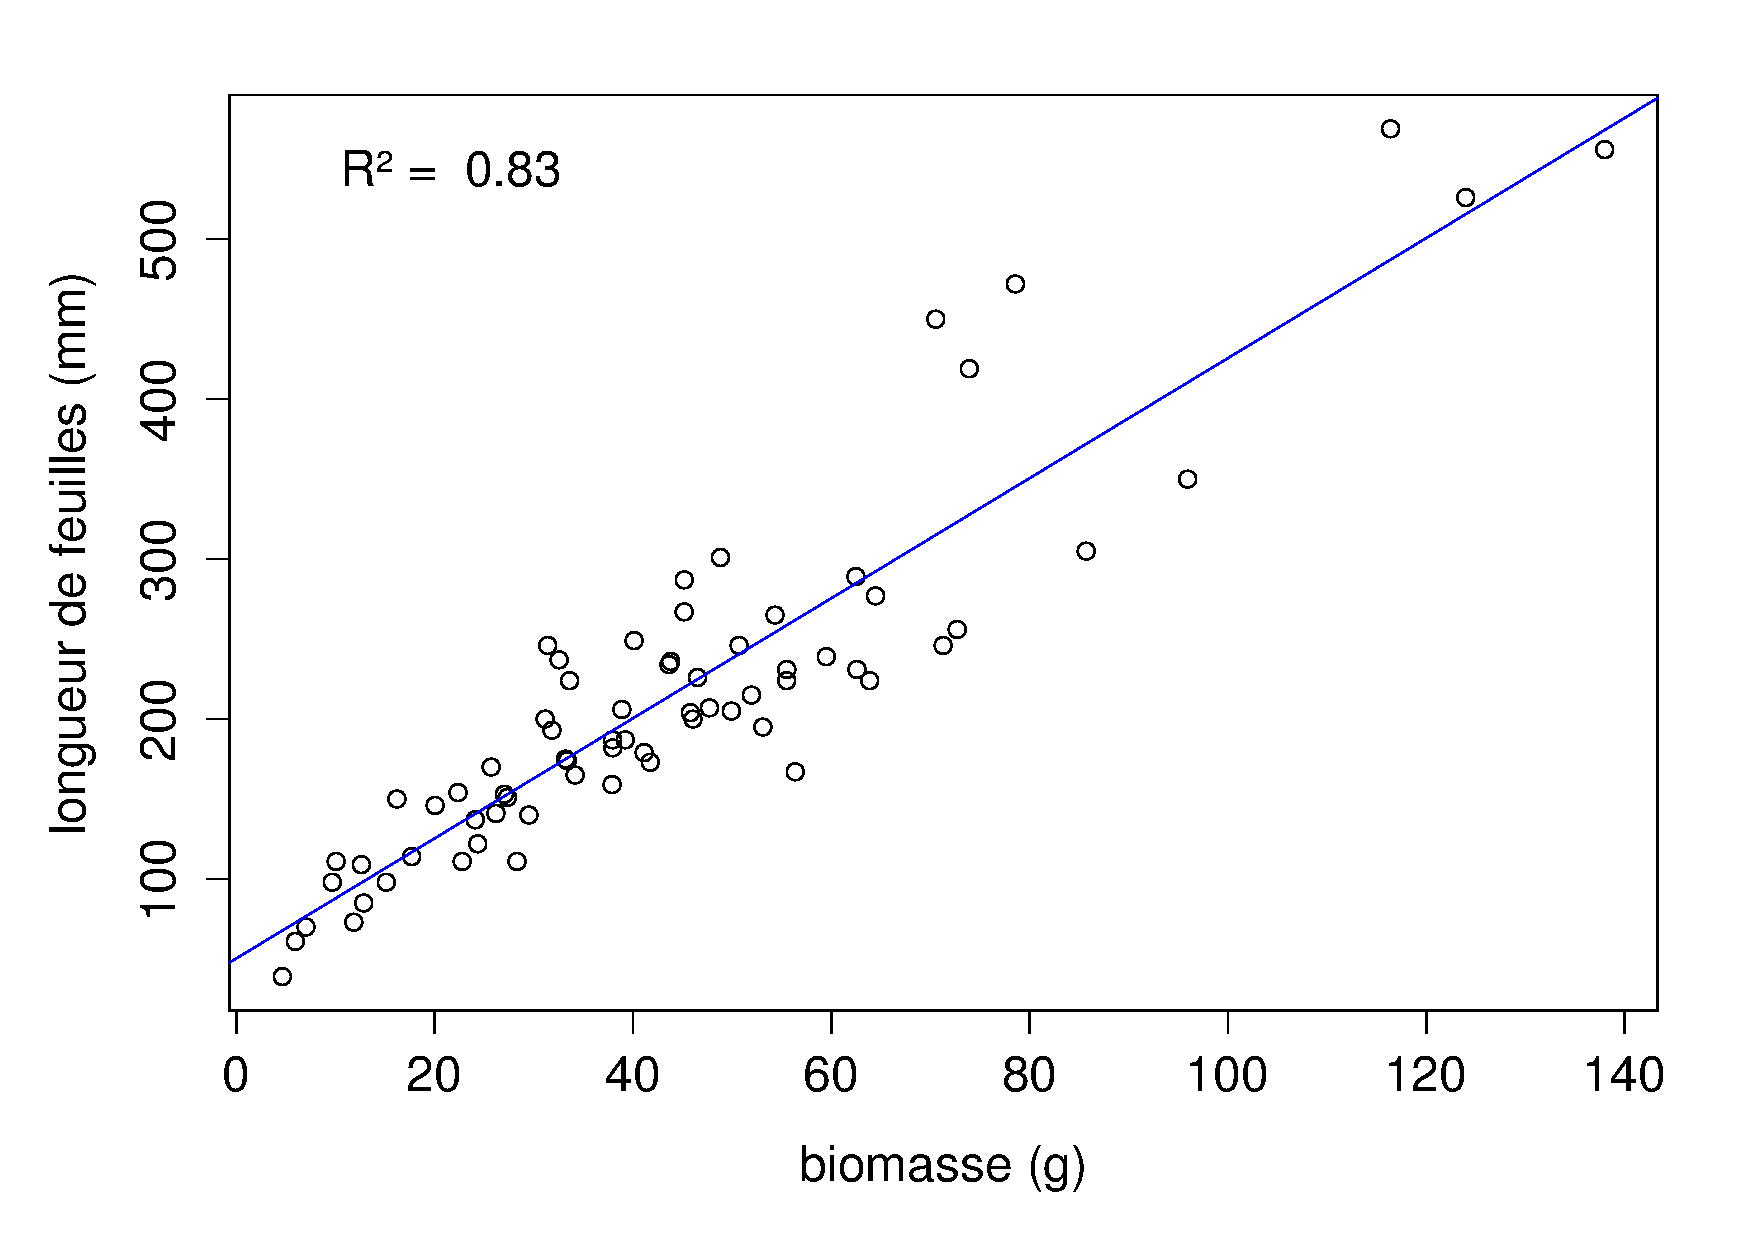
\includegraphics[width=\textwidth]{chap2/mol_lon_bioM}
		\caption{Eriophorum -- biomasse}
	\end{subfigure}
	
	
	\begin{subfigure}[t]{0.5\textwidth}
		\centering
		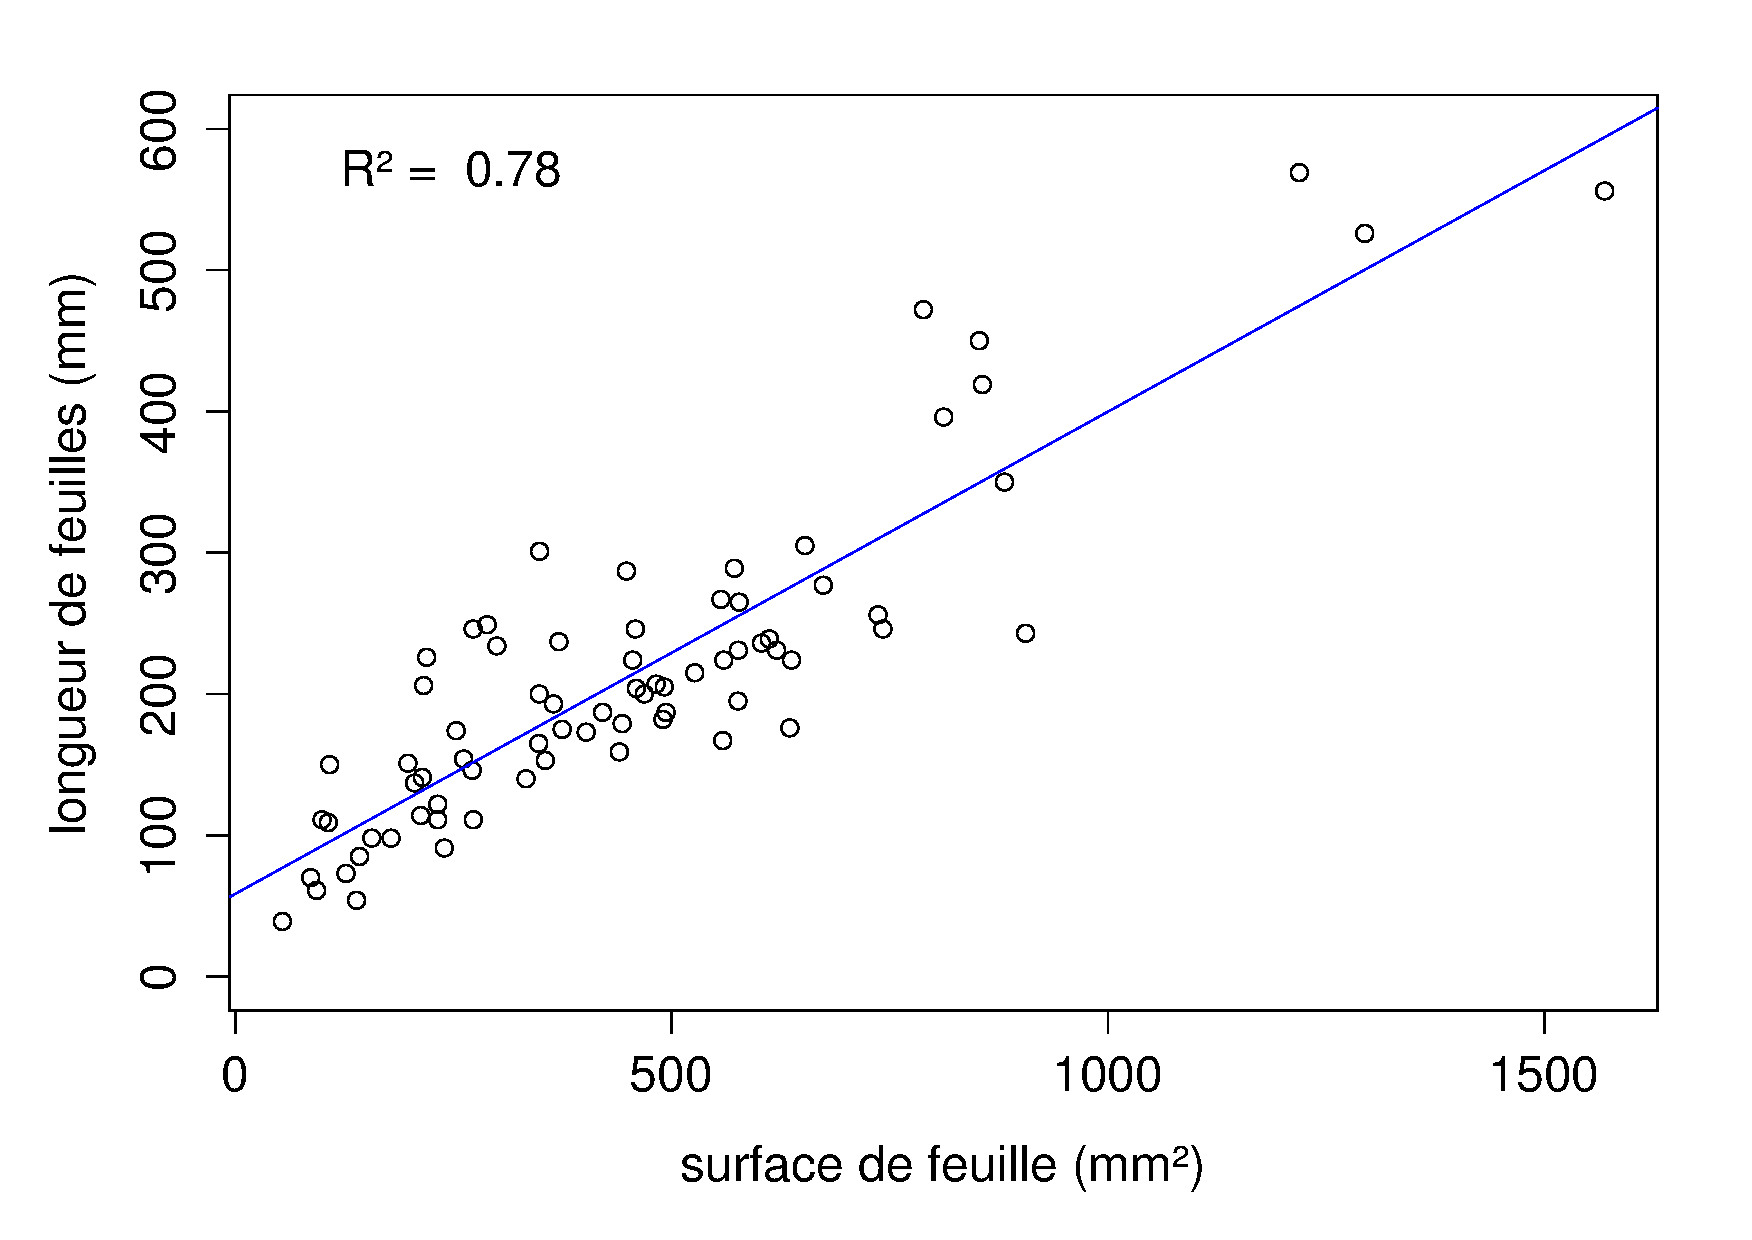
\includegraphics[width=\textwidth]{chap2/mol_lon_surf}
		\caption{Molinia caerulea -- surface}
	\end{subfigure}%
	\begin{subfigure}[t]{0.5\textwidth}
		\centering
		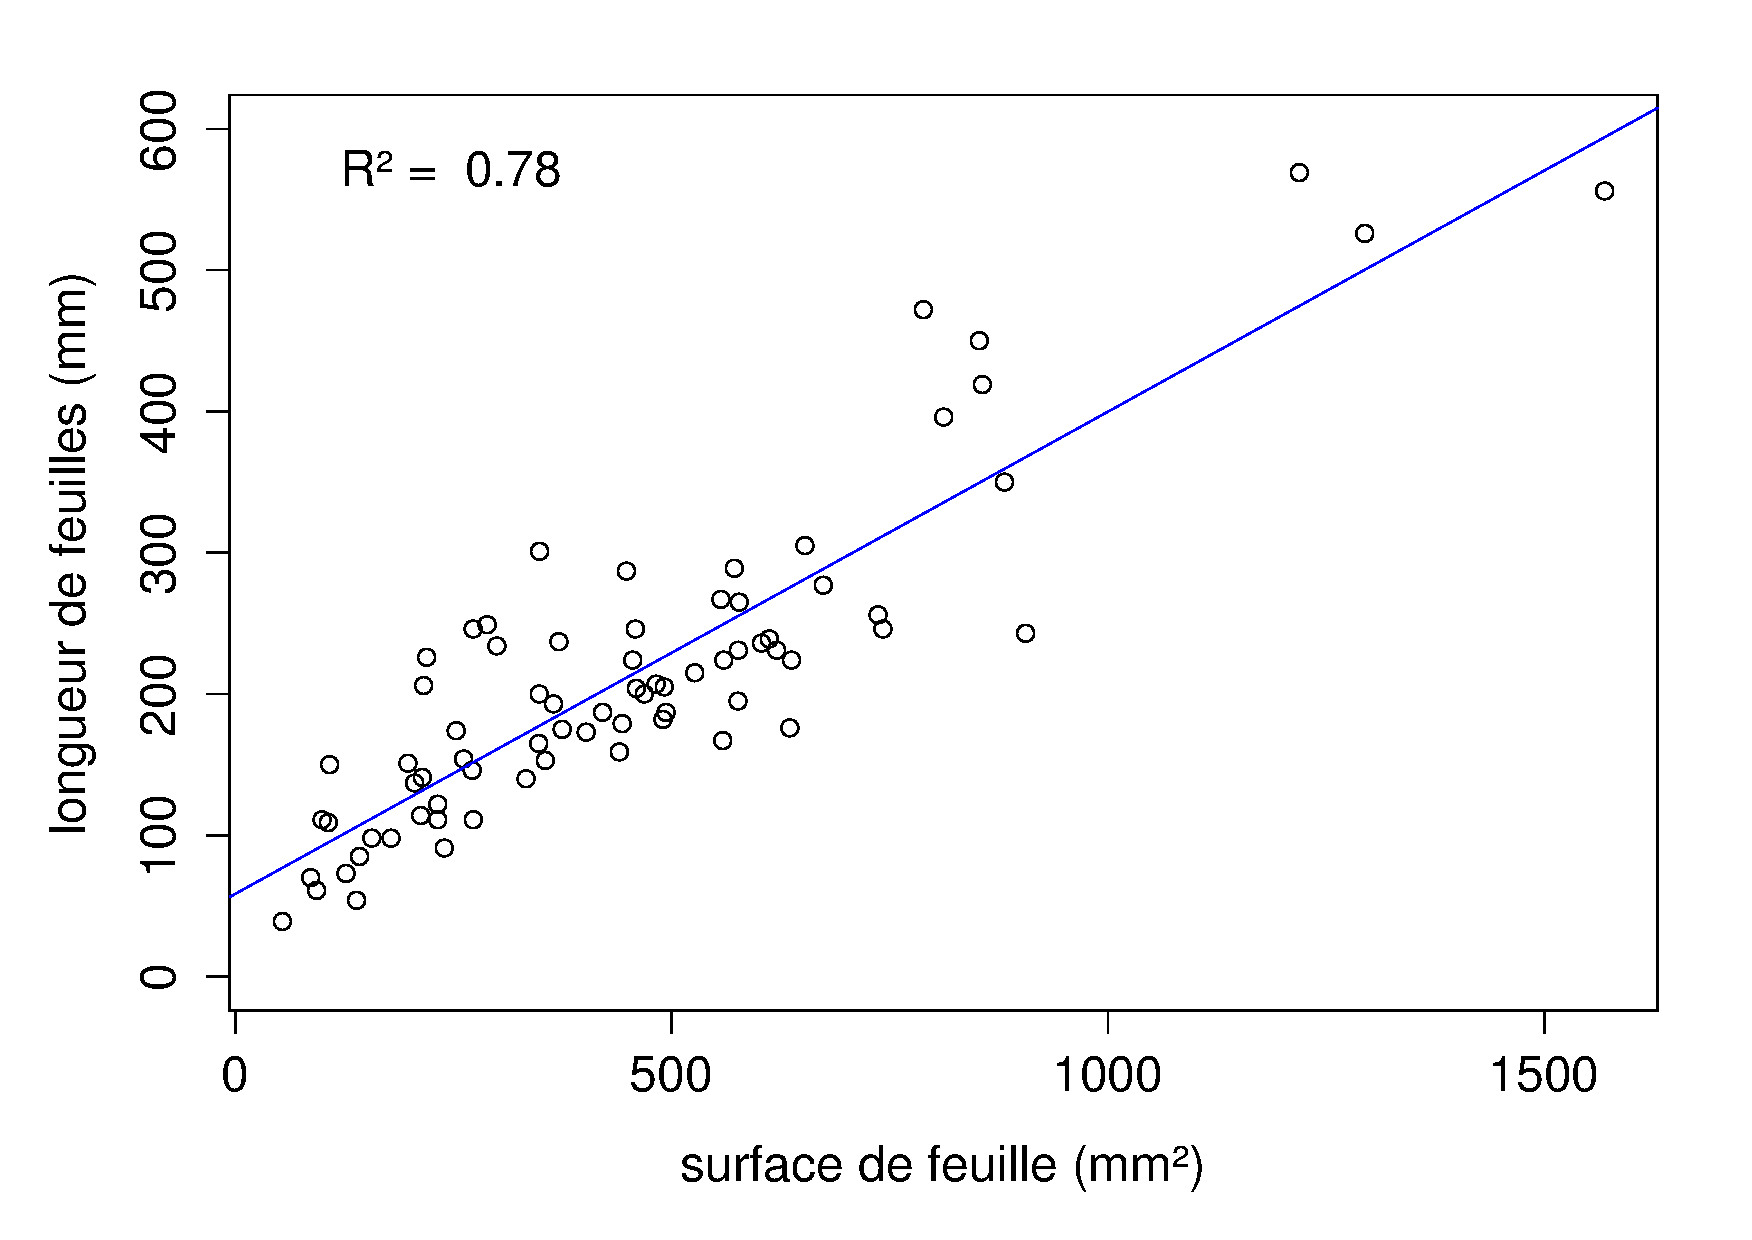
\includegraphics[width=\textwidth]{chap2/mol_lon_surf}
		\caption{Eriphorum -- surface}
	\end{subfigure}
%    \caption{Caption place holder}
\caption{Calibration de la biomasse herbacées pour \textit{molinia Caerulea} (a), pour \textit{eriophorum} (b) et de la surface de feuille pour \textit{molinia Caerulea} (c), pour \textit{eriophorum} (d) en fonction de la hauteur}
\label{fig:cal_herb}
\end{figure}


%\begin{figure}
%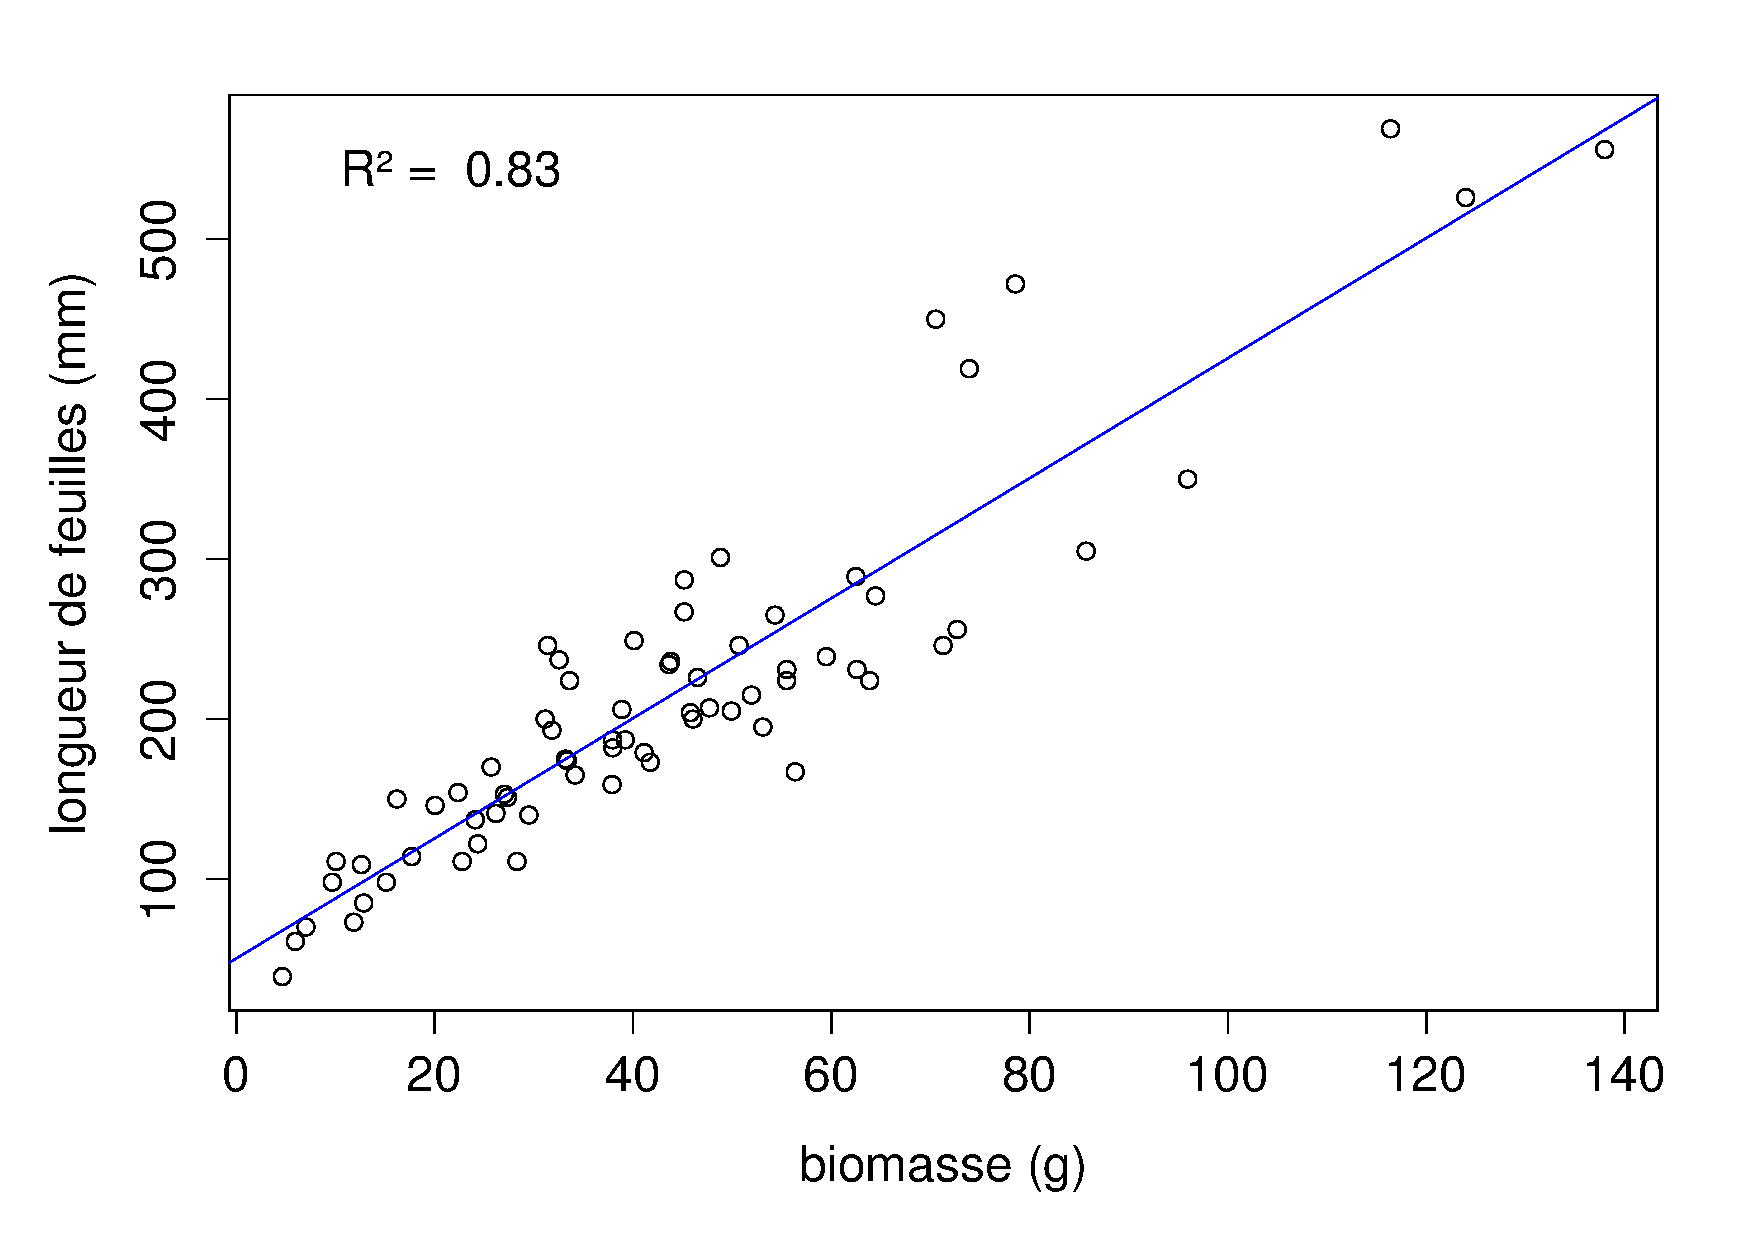
\includegraphics[width=.5\textwidth]{chap2/mol_lon_bioM}
%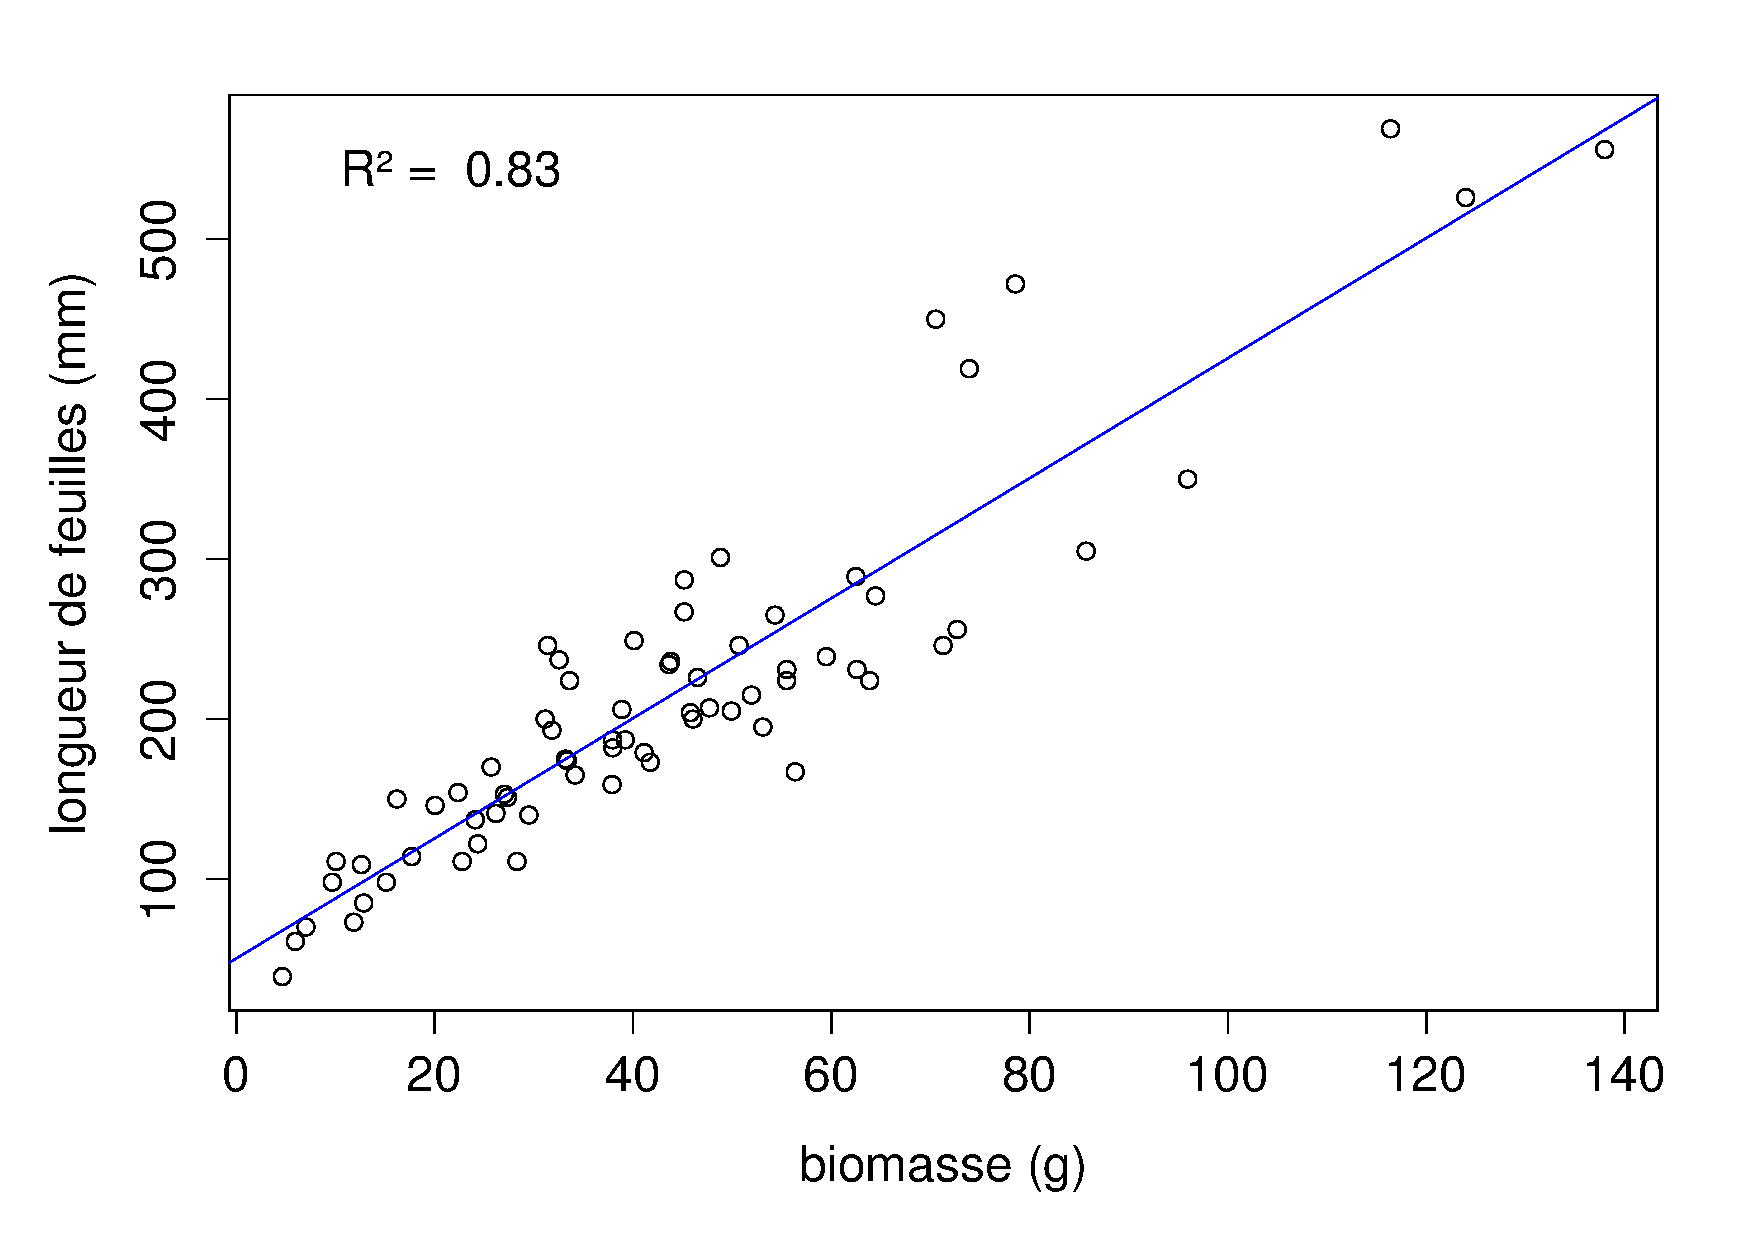
\includegraphics[width=.5\textwidth]{chap2/mol_lon_bioM}
%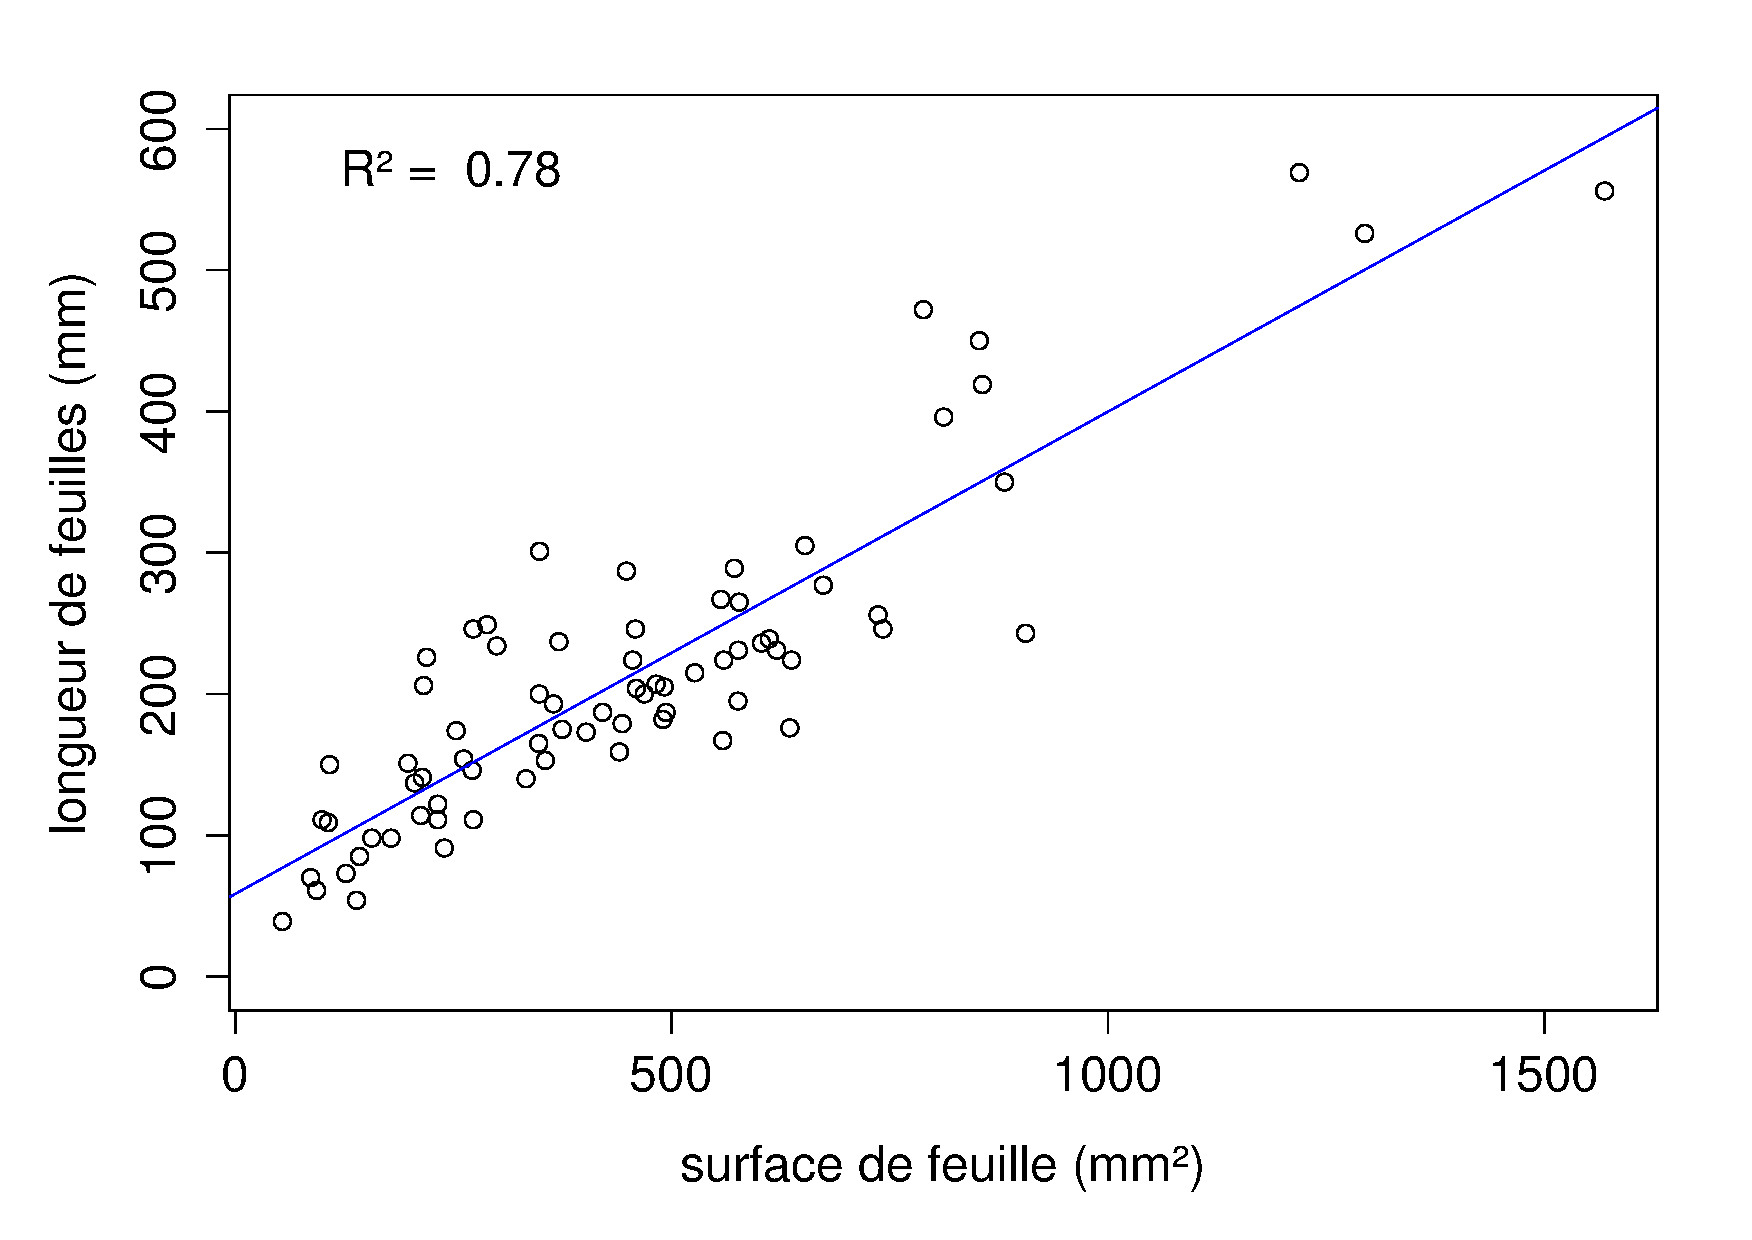
\includegraphics[width=.5\textwidth]{chap2/mol_lon_surf}
%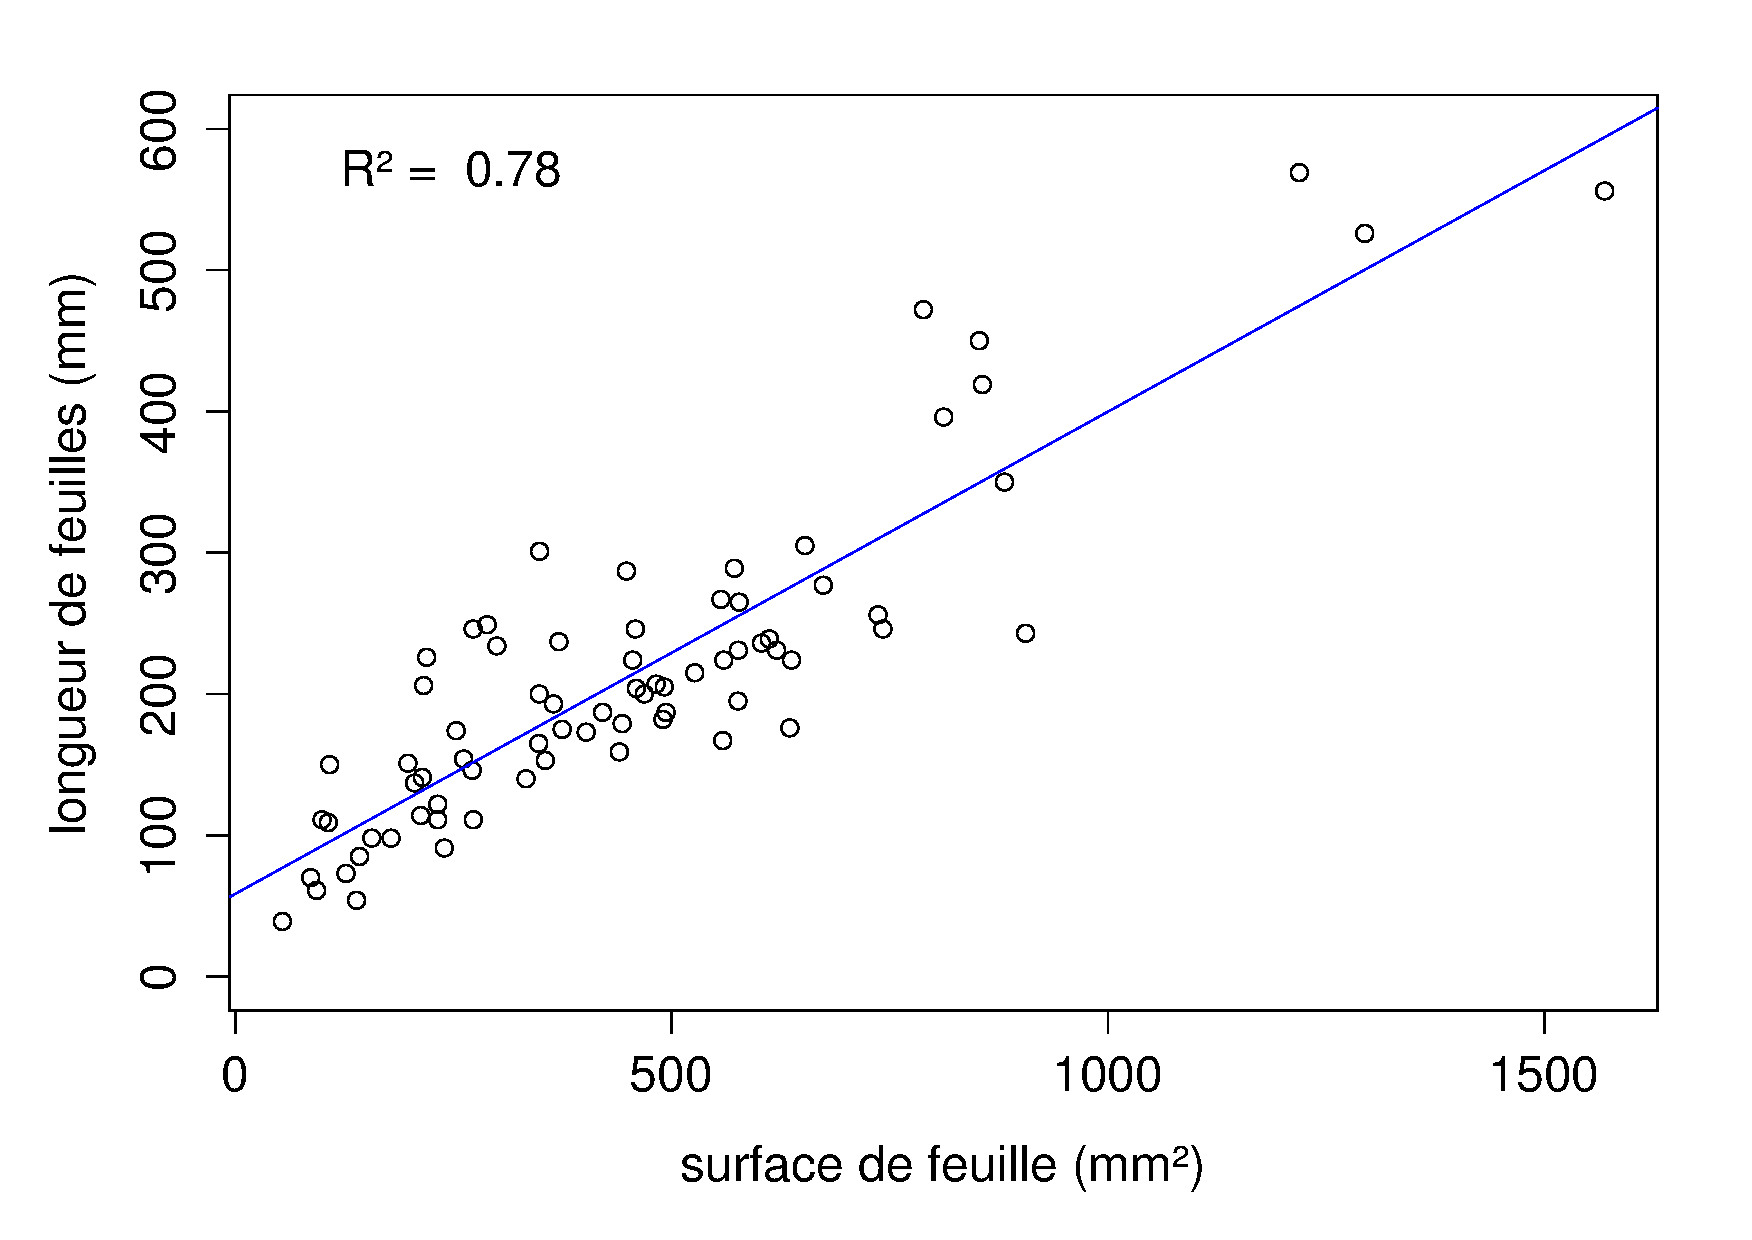
\includegraphics[width=.5\textwidth]{chap2/mol_lon_surf}
%\caption{Calibration de la biomasse herbacées pour \textit{molinia Caerulea} (a), pour \textit{eriophorum} (b) et de la surface de feuille pour \textit{molinia Caerulea} (c), pour \textit{eriophorum} (d) en fonction de la hauteur}
%\label{fig:cal_herb}
%\end{figure}